\documentclass[11pt,twoside,a4paper,BCOR8.25mm,DIV10,headsepline,footsepline,]{scrbook}
%------------------------------------------------------------------------------
%- PAKETE
%------------------------------------------------------------------------------
	%DIN A4
		\usepackage{a4}   

	%Fancy headers
		\usepackage{fancyhdr}
	
	%Sprache einstellen (Inhaltsverzeichnis, ...)
		\usepackage[english,ngerman]{babel} %american,italian,german
	
	%Euro Zeichen
		\usepackage{eurosym}	
		
		\usepackage[bookmarks=true,
					bookmarksopen=true,
   					% Lesezeichen ausgeklappt
					bookmarksnumbered=true,
					colorlinks=true,
				   	%Einf�rbung von Links
					linkcolor=black
					% Linkfarbe: schwarz					
					]
				    % Anzeige der Kapitelzahlen am Anfang der Namen der Lesezeichen
				   {hyperref}
		
	% Vereinfachtes Eingeben von Leerschl�gen hinter Shortcut-Commands
	% Beispiel: \newcommand{\DNA}{desoxyribose nucleid acid\xspace}
		\usepackage{xspace}
	
	%Sortierte Literaturverweise
		\usepackage{cite}
	
	%Grafiken
		\usepackage{float} %Float-Handling mit Schalter H (gleiche Position wie im Skript)
		%\usepackage{flafter} %Verhindert Figuren vor ihrer ersten Referenz
		\usepackage{placeins} %Barriere f�r Float-Umgebungen erzeugen mit \FloatBarrier
	
	%Verbessertes Beschriften mir div. Optionen
		\usepackage{caption}
	
	%Zusaetzliche Symbole und Schriften (ams: american mathematical soc)
		\usepackage{amssymb}
		%\usepackage{amstext}
		%\usepackage{amsfonts}
		%\usepackage{amsbsy}
		%\usepackage{amscd}
		%\usepackage{latexsym}

	%Text Companion fonts which provide many text symbols (such as baht, bullet, copyright, musicalnote, onequarter, section, and yen) in the TS1 encoding.
		\usepackage{textcomp}
	
	%Drehen von Text, Tabellen, Seiten
		%\usepackage{rotating}
	
	%including graphics files, rotating parts of a page, and scaling parts of a page
		\usepackage{graphicx}
	
	%Nice drawing package
		%\usepackage{tikz}               
	
	%besserer eps import: \eps import ERSETZEN durch \epsfig
		\usepackage{epsf}
	
	%Farbunterst�tzung (ausserhalb der Bilder)
		\usepackage{color}
	
	%Postcript einbinden, wobei Text ersetzt werden kann
		%\usepackage{psfrag}
	
	%F�r den Index
		\usepackage{makeidx}
		\makeindex %Muss vor begin{document}, sonst passiert nix
	
	%Erleichterungen f�rs Deutsche inkl Silbentrennung
		%\usepackage{german}
	
	%Ensure minimal spacing of table cells (http://www.ctan.org/tex-archive/help/Catalogue/entries/cellspace.html)
		\usepackage{cellspace}
	
	%Direkte Eingabe von Umlauten mit Angabe von Schriftsatz
	%in Kombination mit 'german' sind jetzt � direkt erlaubt!
		\usepackage[latin1]{inputenc}
	
	%Source code Listings 
		\usepackage{listings}
	
	%Darstellung von Algorithmen
		\usepackage{algorithm}
		\usepackage{algorithmic}
	
	%Subfigures
		\usepackage{subfigure}

%-- Fieser Hack f�r Subfigures (braucht man, um lstlistings im Subfigures zu nutzen)
\newbox\subfigbox
\makeatletter
\newenvironment{subfloat}
{\def\caption##1{\gdef\subcapsave{\relax##1}}%
\let\subcapsave\@empty
\setbox\subfigbox\hbox
\bgroup}
{\egroup
\subfigure[\subcapsave]{\box\subfigbox}}
\makeatother
	
	%Automatically adds the bibliography and/or the index and/or the contents, etc., to the Table of Contents listing.
		%\usepackage[nottoc]{tocbibind} %,notlot,notlof
	
	%St Mary Road symbols for theoretical computer science.
		%\usepackage{stmaryrd}
	
	%URL Darstellung
		\usepackage{url}

	%PDF und Standard Latex Unterscheidung
		\usepackage{ifpdf} 

	%Fancy verbose environments
		\usepackage{fancyvrb}	

	%Abk�rzungsverzeichnis
		\usepackage{nomencl}
		  \let\abbrev\nomenclature
		  \renewcommand{\nomname}{Abk�rzungsverzeichnis}
		  \setlength{\nomlabelwidth}{.25\hsize}
		  \renewcommand{\nomlabel}[1]{#1 \dotfill}
		  \setlength{\nomitemsep}{-\parsep}
		  \makenomenclature

	  \newcommand{\abk}[2]{#1\abbrev{#1}{#2}}
				
	%With \usepackage{ulem}, you have the following new commands:
		%    * \uline{important} underlined text
		%    * \uuline{urgent} double-underlined text
		%    * \uwave{boat} wavy underline
		%    * \sout{wrong} line drawn through word
		%    * \xout{removed} marked over with //////.
		%    * {\em phasized\/} and \emph{asized} In LaTeX, by default, these are underlined; use \normalem or [normalem] to restore italics
		%    * \useunder{\uwave}{\bfseries}{\textbf} use wavy underline in place of bold face 
		%Note that this package changes \em and \emph to be underline. To change this behavior back to normal, use the \normalem command, for example
		%\usepackage{ulem}
		%\normalem
		%\usepackage[normalem]{ulem}

	  %\newcommand{\markup}[1]{\uline{#1}}	

	% package to customize the three basic lists (enumerate, itemize and description) 
	% by means of a set of parameters, and to clone them to define new "logical" lists.
		\usepackage{enumitem}
		\setitemize{enumsep=-3pt}
		\setitemize{itemsep=-3pt}

	%Definitionen
		\usepackage{theorem}
		\newcounter{theorem}
		\newtheorem{definition}[theorem]{Definition}

	%Zitate
		\newcounter{quotectr}
		\newtheorem{myquote}[quotectr]{Zitat}

%------------------------------------------------------------------------------
%- Layout
%------------------------------------------------------------------------------

	%Tiefe des Inhaltsverzeichnisses und der Nummerierung der Kapitel
		\setcounter{secnumdepth}{2}
		\setcounter{tocdepth}{2}

	%Call this after each chapter to avoid headlines on empty pages
		\newcommand{\chapterfin}{\clearpage{\pagestyle{empty}\cleardoublepage}}
		\newcommand{\sectionfin}{\clearpage{\pagestyle{empty}\cleardoublepage}}

	% Listings schoen machen 
		\renewcommand*\ttdefault{txtt}
	
		\lstset{%
		  breaklines=true,
		  basicstyle=\ttfamily\footnotesize,%
		  moredelim=[is][\fontseries{lt}\bfseries]{|}{|},%
		  captionpos=b,%
		  numbers=left,%
		  tabsize=1,%
		  numberstyle=\tiny,%
		  numbersep=6pt,%
		  frame=lr,%
		  framesep=0pt,%
		  framexleftmargin=5pt,%
		  framextopmargin=0pt,%
		  framexbottommargin=0pt,%
		  xleftmargin=15pt,%
		  xrightmargin=15pt,%
			abovecaptionskip=0pt,%
			belowcaptionskip=-0pt,%
		}	
		
		\lstdefinelanguage{XMLSchema}
			{morekeywords={schema,element,annotation,appinfo,complexType,simpleType,choice,all,sequence},		
			sensitive=true,
%			morecomment=[l]{//},
%			morecomment=[s]{/*}{*/},
			morestring=[b]",
		}
		
		\lstdefinelanguage{ASN1}
			{morekeywords={},		
			sensitive=true,
%			morecomment=[l]{//},
%			morecomment=[s]{/*}{*/},
			morestring=[b]",
		}
		
	
	% Font
	%
	%	Danach muss man die Standardschriftart setzen mit dem Befehl \fontfamily{abr}\selectfont, 
	% der f�r das gesamte restliche Dokument gilt, oder mit {\fontfamily{abr}\selectfont Some Text} 
	% um nur den eingeklammerten Bereich zu betreffen. abr ist die Abk�rzung f�r die Schriftart. Die 
	% h�ufigsten sind ptm (Times), phv (Helvetica), pcr (Courier), pbk (Bookman), pag (Avant Garde), 
	% ppl (Palatino), bch (Charter), pnc (New Century Schoolbook), pzc (Zapf Chancery), put (Utopia ).

	% Sch�nerer tt font:
		%\renewcommand{\ttdefault}{pcr}
		%\selectfont
	
	% Times
		%\usepackage{times}
		
	%	Helvetica
			%\usepackage{helvet}
			%\renewcommand{\familydefault}{\sfdefault}
			%\renewcommand{\familydefault}{phv}
			%\fontfamily{abr}\selectfont
			
	%	Courier
			%\usepackage{courier} \raggedright
			%\renewcommand{\familydefault}{\ttdefault}
	
	% Absatzformatierungen:
	% Keeps the distance between paragraphs constant
		\setlength{\parskip}{1.5ex plus 0.0ex minus 0.0ex}
		\setlength{\parindent}{0pt}
	
	% Modify the placement of figures: from faq source: You can adjust the cut-off value if you like, 
	% but it makes no sense to go higher than .95 (LaTeX's default value is only .5). Also, the first 
	% 3 values should be equal, and the last should be 1 - \floatpagefraction.  Otherwise, you are 
	% likely to get floats flushed to the end. 
		\renewcommand{\floatpagefraction}{0.9}
		\renewcommand{\topfraction}{0.9}
		\renewcommand{\bottomfraction}{0.9}
		\renewcommand{\textfraction}{0.1}
		\renewcommand{\textfloatsep}{5mm}
	
	% Zeilenabstand
		\renewcommand{\baselinestretch}{1.0}

	% Fancyheaders 	
		\fancyhf{} % Delete all fields
		%\fancyhead[EL,OR]{\thepage}
		\fancyhead[EL]{\nouppercase{\leftmark}}
		\fancyhead[OR]{\nouppercase{\rightmark}}
		\fancyfoot[EL,OR]{\thepage}	
		
	% Itemize look and feel
		\renewcommand{\labelitemi}{\rule[+0.9mm]{2.7pt}{2.7pt}}
		\renewcommand{\labelitemii}{--}
		%\renewcommand{\labelitemiii}{}
		%\renewcommand{\labelitemiv}{\#}	

	% Floats richtig benennen:
		%\floatname{algorithm}{Algorithm}
		%\renewcommand{\listalgorithmname}{Algorithmen}
		
%------------------------------------------------------------------------------
%- Textbausteine
%------------------------------------------------------------------------------

	%Helpers
		\newcommand{\todo}[1]				{{\em [#1]}\marginpar{{\bf [!!!]}} }
		
		\newcommand{\eigenname}[1]	{{\em #1}}
		
	%Deutsch
		\newcommand{\figref}[1]{Abbildung~\ref{fig:#1}}
		\newcommand{\tabref}[1]{Tabelle~\ref{tab:#1}}
		\newcommand{\equref}[1]{Gleichung~\ref{equ:#1}}
		\newcommand{\chapref}[1]{Kapitel~\ref{cha:#1}}
		\newcommand{\appref}[1]{Anhang~\ref{cha:#1}}
		\newcommand{\secref}[1]{Abschnitt~\ref{sec:#1}}
		\newcommand{\lstref}[1]{Listing~\ref{lst:#1}}
		\newcommand{\algref}[1]{Algorithmus~\ref{alg:#1}}
		\newcommand{\ssecref}[1]{Unterabschnitt~\ref{ssec:#1}}
		\newcommand{\quoteref}[1]{Zitat~\ref{quote:#1}}

	%Englisch	
		%\newcommand{\figref}[1]		{Figure~\ref{fig:#1}}
		%\newcommand{\tabref}[1]		{Table~\ref{tab:#1}}
		%\newcommand{\equref}[1]		{Equation~\ref{equ:#1}}
		%\newcommand{\algref}[1]		{Algorithm~\ref{alg:#1}}
		%\newcommand{\defref}[1]		{Definition~\ref{def:#1}}
		%\newcommand{\quoteref}[1]	{Quote~\ref{quote:#1}}
		
		%\newcommand{\chapref}[1]	{Chapter~\ref{cha:#1}}
		%\newcommand{\appref}[1]		{Appendix~\ref{cha:#1}}
		%\newcommand{\secref}[1]		{Section~\ref{sec:#1}}
		%\newcommand{\ssecref}[1]	{Section~\ref{ssec:#1}}
		%\newcommand{\sssecref}[1]	{Section~\ref{sssec:#1}}
		
	% REDEFINE UGLY STUFF
		\renewcommand{\leq}		{\leqslant}
		\renewcommand{\geq}		{\geqslant}
		\renewcommand{\epsilon}	{\varepsilon}
		\newcommand{\musec}		{$\mu sec$\xspace}
		\newcommand{\muW}		{$\mu W$\xspace}
		\newcommand{\plusminus}	{$\pm $\xspace}
	
%------------------------------------------------------------------------------
%- Worttrennung
%------------------------------------------------------------------------------
	
	%\hyphenation{Ge-samt-ozon}	
	\hyphenation{name-space}	
	\hyphenation{name-spaces}	
	\hyphenation{ge-samten}	
			
%------------------------------------------------------------------------------
%- Grafiken
%------------------------------------------------------------------------------

	\ifpdf
	  \DeclareGraphicsExtensions{.jpg,.pdf,.png}   % for pdftex driver
	\else
	  \DeclareGraphicsExtensions{.eps}             % for dvips driver
	\fi
	
	% Vereinfacht die Einbettung von Grafiken
	% Beispiel: \myfig[5cm]{psdatei}{�bersicht �ber das Gesamtsystem}
	\newcommand{\myfig}[3][\columnwidth]
	{
	 \begin{figure}[htbp]
		 \begin{center}
			 \includegraphics[width=#1]{img/#2}
			 \caption{#3}
			 \label{fig:#2}
		 \end{center}
	 \end{figure}
	}
	
	\newcommand{\myfigtwo}[4][\columnwidth]
	{
		 \begin{figure}[htbp]
				\begin{center}
				  \mbox
				  {
				    \subfigure[#2] 
				    { \includegraphics[width=.45\columnwidth]{img/#1-a} \label{fig:#1-a} } 
				    \quad
				    \subfigure[#3]
				    { \includegraphics[width=.45\columnwidth]{img/#1-b} \label{fig:#1-b} }
			    }
				  \caption{#4}
					\label{fig:#1}
				\end{center}
			\end{figure}
	}
	
	\newcommand{\myfigthree}[5][\columnwidth]
	{
		 \begin{figure}[htbp]
				\begin{center}
				  \mbox{
				    \subfigure[#2]
				    {
				    	\includegraphics[width=.3\columnwidth]{img/#1-a}
				    	\label{fig:#1-a}
				    } 
				    \subfigure[#3]
				    {
							\includegraphics[width=.3\columnwidth]{img/#1-b}
				    	\label{fig:#1-b}
				    }
				    \subfigure[#4]
				    {
							\includegraphics[width=.3\columnwidth]{img/#1-c}
				    	\label{fig:#1-c}
				    }
			    }	
				  \caption{#5}
					\label{fig:#1}
				\end{center}
			\end{figure}
	}
	
	\newcommand{\myfigfour}[6][\columnwidth]
	{
		 \begin{figure}[htbp]
				\begin{center}
				  \mbox
				  {
				    \subfigure[#2] 
				    { \includegraphics[width=.45\columnwidth]{img/#1-a} \label{fig:#1-a} } 
				    \quad
				    \subfigure[#3]
				    { \includegraphics[width=.45\columnwidth]{img/#1-b} \label{fig:#1-b} }
			    }
				  \mbox
				  {
				    \subfigure[#4] 
				    { \includegraphics[width=.45\columnwidth]{img/#1-c} \label{fig:#1-c} } 
				    \quad
				    \subfigure[#5]
				    { \includegraphics[width=.45\columnwidth]{img/#1-d} \label{fig:#1-d} }
			    }
			    
				  \caption{#6}
				\label{fig:#1}
				\end{center}
			\end{figure}
	}
	


% F�r das Abk�rzungsverzeichnis
\usepackage[printonlyused]{acronym}  
\usepackage{savefnmark}

%Um die Abkuerzungen zu ermoeglichen:
% 	makeindex.exe thesis.nlo -s nomencl.ist -o thesis.nls
%   als Postprocessor in Texniccenter einrichten

% Nette Hinweise zum LaTexen einer Diss: 
% - http://iacweb.ethz.ch/en/various/Mittelbau/disslatex.html
% - http://www.zib.de/pfetsch/Diss-Styles/
% - http://www2.informatik.hu-berlin.de/~nlohmann/arbeit/koma.html

% Hiermit kann man festlegen, dass immer nur ein bestimmter Teil �bersetzt wird
%\includeonly{1-einleitung}

\begin{document}
\selectlanguage{ngerman}
\frontmatter

%---------------------------------------------------------------------------
% Frontpage
%---------------------------------------------------------------------------
	%---------------------------------------------------------------------------
% Frontpage
%---------------------------------------------------------------------------

\begin{titlepage}

\title{Entwicklung einer Android Anwendung zum transparenten und anonymen
Sammeln von Sensordaten}
\author{Malte Legenhausen}

\let\footnotesize\small
	\let\footnoterule\relax
	\null
	\vfil
	\vskip 30pt
	\begin{center}
		{\LARGE
		  {
\includegraphics[width=80mm]{grafiken/Logo_Inst_Telematik_cropped.pdf}
			\\
			\vskip 20pt
			\Large Universit"at zu L"ubeck}\\
			Institut f"ur Telematik\\[2cm]
			{\Large Masterarbeit}\\ [2cm]
			Entwicklung einer Android Anwendung zum transparenten und anonymen Sammeln
			von Sensordaten \par}%
		\vskip 5em
		{\large \lineskip .75em
		\begin{tabular}[t]{c}
			{\Large von}\\[.5em]
			{\Large Malte Legenhausen}\\[7em]
			{\bf Aufgabenstellung und Betreuung:}\\[.5em]
			Prof.\ Dr.\ S.\ Fischer\\
			Dr.-Ing.\ Dennis\ Pfisterer\\
			M.\ Sc.\ Daniel\ Bimschas
		\end{tabular}
		\par}%
		\vfill 
		{\large
			L�beck, den \today
			\par}%
	\end{center}
	\par
	% thanks
	\vfil
	\null
\end{titlepage}

\cleardoublepage

% Erklaerung
\newpage
\vspace*{7cm}
\centerline{\bf Erkl"arung}

\vspace*{1cm}
Ich versichere, die vorliegende Arbeit selbstst"andig und nur unter Benutzung
der angegebenen Hilfsmittel angefertigt zu haben.

\vspace*{3cm}
L�beck, den \today 

\pagestyle{headings}

\cleardoublepage

% Kurzfassung und Abstract

\centerline{\bf Kurzfassung}
\bigskip
In der heutigen Zeit erfassen Smartphones sehr viele personenbezogene Daten
(z.B. Standort, Benutzerverhalten) �ber ihren Besitzer. Diese Daten besitzen
einen relativ hohen Wert f�r �ffentliche Einrichtungen und die Industrie. In den
meisten F�llen, werden diese Daten ohne das Wissen des Benutzers, aber nur an
wenige externe dritte �bertragen (z.B. Mobilfunkanbieter, Google, Apple). Die in
dieser Arbeit entwickelte L�sung, soll eine Android Anwendung darstellen, die
das transparente und anonyme Sammeln von Sensordaten erm�glicht. Die Anwendung
stellt dazu ein Erweiterungssystem bereit, das die kontrollierte Ausf�hrungs von
Plug-Ins erlaubt. Plug-Ins k�nnen von externen Einrichtung entwickelt
werden und beliebige Daten �ber den Benutzer sammeln. Der Benutzer erh�lt die
M�glichkeit zu jedem Zeitpunkt alle gesammelten Daten einzusehen und kann selbst
bestimmen welche Daten �bertragen werden sollen und welche nicht. Durch diese
Anwendung soll der Benutzer die Kontrolle �ber seine Daten wiedererlangen und es
auch anderen Instritutionen erm�glichen personenbezogene Daten zu sammeln.

%
\vskip 3cm
%

\centerline{\bf Abstract}
\bigskip
Today's smartphones collect a high amount of personalized data (e.g. position,
user behaviour) from the owner. This data has a relativly high value for public
institutions and the industry. But in most cases this data is transmitted
without the knowledge of the user only to few external thrid parties (e.g. 
provider of mobile telecom services, Google, Apple). The solution developed in
this thesis is an Android application that is able to collect personalized data
in a transparent and anonymous way. The application provides an extensible
system that allows the controlled executions of plug-ins. Plug-Ins can be
developed by external institutions that can collect arbitary data about the
user. At any point in time the user has the possibility to review all
the collected data and can decide which data is transfered and which not.
Through this application the user should get back control over his data and
enable other institutions to collect personalized data.

\cleardoublepage

%---------------------------------------------------------------------------
% Inhaltsverzeichnis
%---------------------------------------------------------------------------
	\tableofcontents
	\cleardoublepage

%---------------------------------------------------------------------------
% Der eigentliche Inhalt
%---------------------------------------------------------------------------
	\mainmatter
	\pagestyle{fancy}
	
	\chapter{Einleitung}
\label{cha:einleitung}
Diese Masterarbeit�stellt die Abschlussarbeit des�Autors zum Master of Science
dar, die im�Rahmen�des�Studienganges�Informatik an�der Universit�t zu L�beck
absolviert wurde.�Die Themenbearbeitung�fand�an der Universit�t zu L�beck im
\acf{itm}�statt. Der�Themenschwerpunkt�dieser Masterarbeit�ist�die Entwicklung
einer Android Anwendung zum transparenten und anonymen Sammeln von Sensordaten.

Diese Anwendung soll einige Nachteile der bisherigen Ans�tze der mobilen
Datenerfassung l�sen, die auf potenziell pers�nliche Daten eines Smartphone-Benutzers
zugreifen. Denn heutzutage werden �ber einen Benutzer, eine
Vielzahl unterschiedlicher Daten gesammelt. Dies reicht von der aktuellen Position, bis
hin zu den Gewohnheiten wie ein Benutzer sein Smartphone verwendet. In vielen
F�llen wei� ein Smartphone-Benutzer nicht, welche Anwendung welche Daten �ber
ihn sammelt bzw. dass dies �berhaupt geschieht. Auch fehlt eine M�glichkeit die
gesammelten Daten einzusehen, geschweige denn einer �bertragung der Daten zu
widersprechen. Ob bei der �bertragung eine Anonymisierung der Daten
stattfindet, liegt ebenfalls in der Hand des Anwendungsherstellers.

Diese Umst�nde f�hren dazu, dass sich viele Smartphone-Benutzer ihrer Daten
entmachtet f�hlen und somit das Misstrauen in Anwendungen der mobilen
Datenerfassung steigt. Dies kann zu einem Problem werden, wenn immer weniger
Benutzer Daten (ob personenbezogenen oder nicht) freigeben wollen,
obwohl der Bedarf nach solchen Daten in einer Vielzahl von Industrie und
Forschungsprojekten steigt.

Motivation ist es daher, eine vertrauensw�rdige Plattform zu schaffen, auf der
aufbauend andere Institutionen Anwendungen zum Sammeln von Sensordaten
entwickeln k�nnen. Sensordaten sind im Rahmen dieser Arbeit z.~B. der L�rmpegel
der Umgebung, die aktuelle Position, die verf�gbaren Netzwerkverbindungen oder
die Daten des Beschleunigungssensors. Die Plattform soll dabei dem Benutzer
erm�glichen selbst zu entscheiden, wann welche Daten �ber ihn gesammelt werden
sollen. Transparenz soll der Benutzer dadurch erhalten, dass er zu jedem Zeitpunkt
einsehen kann, welche Daten �ber ihn gesammelt wurden. Des Weiteren soll der
Benutzer auch entscheiden k�nnen, ob die gesammelten Daten �berhaupt an eine andere
Institution freigegeben werden sollen. Anonymit�t soll dadurch erreicht
werden, dass der Zugriff auf eindeutige Benutzerdaten geregelt wird. Diese Daten
k�nnen z.~B. der Name, Telefonnummer oder die Adresse sein.

Ziel ist es die informationelle Selbstbestimmung des Benutzers zu festigen und
somit, auch das Vertrauen in die mobile Datenerfassung zu steigern. Durch dieses
Vertrauen sollen gerade �ffentliche Forschungseinrichtungen die M�glichkeit
erhalten personenbezogene Daten zu sammeln, die z.~B. im Bereich der
St�dte- und Verkehrsplanung neue Erkenntnisse liefern k�nnen.

\section{Verwandte Arbeiten}
Im Folgenden sollen auf �hnliche Arbeiten eingegangen werden, die bereits
einzelne Aspekte der zu entwickelnden Anwendung realisiert haben. 

\subsection{Sensorly}
Bei {\em Sensorly} handelt es sich um eine Android Anwendung, mit der die
Netzwerkabdeckung von Mobilfunknetzen mithilfe von Android-Smartphones ermittelt
wird. Dazu l�dt man sich als Benutzer eine Gratisanwendung aus dem {\em
Android Market} herunter und installiert diese. Nach dem ersten Start sammelt
die Anwendung automatisch im Hintergrund Daten �ber die Netzabdeckung vom gerade
verbundenen Mobilfunkanbieter. Diese Daten werden in regelm��igen Abst�nden an einen
zentralen Server �bermittelt, wo diese Daten mit den Daten anderer Anwender
kombiniert werden, um die Daten anschlie�end in einer Karte auf der
Internetseite \url{sensorly.com} zu visualisieren.

{\em Sensorly} repr�sentiert einen m�glichen Anwendungsfall f�r die zu
entwickelnde Anwendung. Es ist mit {\em Sensorly} aber nicht m�glich die Daten
vor der �bertragung einzusehen oder dieser �bertragung zu widersprechen. {\em
Sensorly} stellt also eine klassische Anwendung zum Sammeln von Sensordaten dar.

\subsection{Flexible Android Permissions}
\acf{flexp} ist eine Anpassung des Android Betriebssystems, die es erm�glicht,
die Rechte die einer Anwendung bei der Installation gegeben werden, nachtr�glich zu
ver�ndern. Ein Benutzer hat also die M�glichkeit nachtr�glich zu bestimmen, auf
welche Ressourcen eine Anwendungen zugreifen darf und auf welche nicht. Um nun
m�gliche Probleme zu vermeiden, die nach dem Rechteentzug auftreten
k�nnen, wird den Anwendungen suggeriert, dass sie trotzdem Zugriff auf die
Ressourcen haben~\cite{flexp}.

\acs{flexp} deckt den Aspekt ab, dass durch diese Anpassung der Benutzer mehr
M�glichkeiten hat, zu entscheiden auf welche Ressourcen (z.~B. die Sensorik),
die Anwendung zugreifen darf. Der Benutzer hat aber hier ebenfalls nicht die
M�glichkeit einsehen, was passiert, wenn ein Recht trotzdem vergeben wurde. Die
Kontrollm�glichkeiten �ber eine Anwendung steigen zwar, die Transparenz bleibt
aber dieselbe.

\subsection{iPhone Tracker}
Der {\em iPhone Tracker} erlaubt die Visualisierung von Daten auf dem Computer,
die durch das Smartphone-Betriebssystem iOS auf dem Apple iPhone erhoben
werden~\cite{iphonetracker}. Diese Daten werden laut Apple dazu verwendet, die
Lokalisierung des Benutzers zu beschleunigen. Die Daten erlauben aber die
einfache Generierung von Bewegungsprofilen. Eine Einsicht dieser Daten ohne
spezielle Programme ist aber nicht m�glich~\cite{applegps}.

Der Fall des {\em iPhone Tracker} zeigt, die Problematik bei fehlender
Transparenz. Dem Benutzer ist nicht bewusst, welche Daten �ber ihn gesammelt
werden. Kommt dieses zutage, bedeutet dies oft ein Vertrauensbruch mit dem
Benutzer. Die zu entwickelnde Anwendung soll nun diese Transparenz als
Standardfunktionalit�t liefern. Anwendungen, die auf dieser aufbauen, m�ssen
sich nur um das eigentliche Sammeln von Daten k�mmern.

\section{Aufbau der Masterarbeit}
Diese Masterarbeit gliedert sich in die folgenden Kapitel:

\begin{itemize}
  \item In der {\bf Anforderungsanalyse} wird die Aufgabenstellung in ihre
  einzelnen Bestandteile zerlegt und Begrifflichkeiten gekl�rt. Dies erlaubt in
  den nachfolgenden Kapiteln die Bearbeitung der in der Aufgabenstellung
  enthaltenden Anforderungen.
  \item Die {\bf Grundlagen} befassen sich mit den verwendeten Technologien.
  Dieses Kapitel besch�ftigt sich zu einem gro�en Teil mit der Android
  Plattform.
  \item Die {\bf Konzeption} beschreibt einen weitestgehenden
  techno\-logie\-unab\-h�n\-gigen Aufbau der Anwendung. Dabei werden die
  Anforderungen in eine Architektur �berf�hrt. Es wird aber auch gekl�rt, ob die
  in den Grundlagen erw�hnten Technologien sich tats�chlich zur Realisierung
  verwenden lassen.
  \item In der {\bf Realisierung} wird die entwickelte Anwendung vorgestellt.
  Dies schlie�t interne Abl�ufe ein, wie auch die Pr�sentation der
  Benutzerschnittstelle.
  \item Der {\bf Leitfaden} dient Entwicklern als Anleitung um ihre Anwendungen
  (Plug-Ins) zu entwickeln und diese auf der Plattform auszuf�hren.
  \item Die {\bf Evaluation} dient als Best�tigung, dass die entwickelte
  Anwendung auch in realen Anwendungsszenarien einsetzbar ist.
  \item Im Kapitel {\bf Zusammenfassung und Ausblick} werden die Ergebnisse der
  Arbeit zusammengefasst und ein abschlie�endes Fazit gegeben.
\end{itemize} 	
	\chapterfin
	\chapter{Anforderungsanalyse}
\label{cha:anforderungsanalyse}
In diesem Kapitel werden die aus der Aufgabenstellung sich ergebenen
Anforderungen genauer analysiert. Es wird dabei gekl�rt, in welchem Umfang die
einzelnen Anforderungen bearbeitet werden m�ssen.

Die sich aus der Aufgabenstellung ergeben Anforderungen sind Transparenz,
Anonymit�t, ein Erweitungssystem, die m�glichkeit der Datenspeicherung, sowie
die regelm��ige �bertragung von Daten an einen Server.

\section{Transparenz}


\section{Anonymit�t}
Anonymit�t beschreibt den Zustand, einer Person oder Gruppe die
nicht identifiziert werden kann. Bei der Art von Anonymit�t
gibt unterscheidet man verschiedene Abstufungen~\cite{anonymitaet}:
\begin{itemize}
  \item formal anonym: Eindeutige Zuordnungsmerkmale (z.B. Namen usw.) sind
  entfernt, die Daten ansonsten unver�ndert (das hei�t leichte Zuordbarkeit der Einheiten).
  \item faktisch anonym: Daten sind nur nur mit unverh�ltnism��igem Zeit- und
  Arbeitsaufwand zuordbar.
  \item komplett anonym: die Zuordnung zu einzelnen Personen ist ausgeschlossen.
\end{itemize}

Im Rahmen der Aufgabenstellung soll eine Anonymisierung der Benutzers
von ``formal anonym'' bis ``faktisch anonym'' erm�glicht werden. Dies bdeutet,
dass es nicht m�glich sein soll, eindeutige Merkmale eines Benutzers zu sammeln (z.B.
IMEI, Telefonnummer) und zum anderen, eine Zuordnung zu realen Personen anhand
der Daten erschwert wird.

Bei der Anonymisierung der Daten ergibt sich aber ein Problem, bei der
zurordbarkeit von einzelnen Datens�tzen, die in regelm��igen Abst�nden an einen
Server �bertragen werden. Werden zwei Datens�tze A und B zu zwei
unterschiedlichen Zeitpunkten �bertragen, ist es nicht m�glich die
Datens�tze A und B einander zuzurodnen. Eine Zuordnung auf dieser Ebene gef�hrte
aber nicht die Anonymit�t der Benutzers. Hierbei ergibt sich nun die Anforderung
eine Verfahren zu entwickeln, dass dieses Problem l�st.

\section{Erweiterungssystem}
Aus der Aufgabenstellung ist zu entnehmen, dass die zu entwickelnde Anwendung,
nur ein Grundger�st darstellen soll. Es soll sich durch Erweitungen erweitern
lassen. Die Anforderung besteht also darin, ein bestehendes Erweitungssystem in
Android zu integrieren, oder ein eigenes zu implementieren.

Anforderungen an das Erweiterungssystem:

\begin{itemize}
  \item Der Benutzer soll die m�glichkeit haben neue Erweiterungen zu
  installieren und zu deinstallieren.
   \item Die Installation neuer Erweiterungen, soll f�r den Benutzer der
   Anwendung m�glichst einfach sein z.B. durch die Bereitstellung eines Markets.
  \item Das Erweiterungssystem soll eine Bibliothek liefern, �ber die es m�glich
  ist neue Erweiterungen m�glichst einfach zu erstellen.
\end{itemize}

\section{Datenspeicherung}
Die von den Erweiterungen gesammelten Daten m�ssen auf dem Ger�t zwischen
gespeichert werden, bevor diese �bertragen werden d�rfen. Der Benutzer soll
n�mlich die M�glichkeit besitzen, sich die gesammelten Daten, vor einer
�bertragung zu kontrollieren. Deswegen ist ein Datenmodell zu entwickeln, dass
es erm�glicht, Daten von beliebigen Erweiterungen zu speichern. Der Entwickler
einer Erweiterung soll dabei aber so wenig wie m�glich bei der Wahl seines
Datenmodell eingeschr�nkt werden.

\section{Daten�bertragung}
Die von den Erweiterungen gesammelten Daten sollen in regelm��igen Abst�nden, an
einen Server �bertragen werden. Dies soll aber nicht automatisch geschehen,
sondern es soll der Benutzer darauf hingewiesen werden, das neue Daten zur
�bermittung bereit stehen. Dadurch soll der Benutzer die m�glichkeit haben vor
einer �bertragung die Daten zu kontrollen. Ist ein Benutzer nicht mit der
�bertragung der Daten einverstanden, so soll diese �bertragung verworfen werden
k�nnen. Des Weiteren soll die M�glichkeit bestehen die �bertragung zu einem
sp�teren Zeitpunkt auszuf�hren. Dies kann der Fall sein, wenn eine �bertragung
z.B. �ber das Mobilfunknetz f�r den Benutzer zu kostenintensiv ist.

F�r die �bertragung der Daten ist ein entsprechendes Datenformat und
�bertragungsprotokoll zu w�hlen. Beim Datenformat ist darauf zu achten ein
Format zu w�hlen, dass einen geringen Overhead aufweist, da die Bandbreite im
mobilen Bereich stark limitiert ist.

Zum Empfangen der Daten ist eine entsprechende Serverkomponente zu entwickeln.
Neben dem Empfang soll die Serverkomponente es erlaubt die empfangenen Daten
weiter zu verarbeiten um sie z.B. in einer Datenbank zu speichern.

	\chapterfin
	\chapter{Grundlagen}
\label{cha:grundlagen}

In diesem Kapitel wird auf die grundlegenden Technologien eingegangen, die zur
Realisierung der Anwendung verwendet wurden.

\section{Mobile Anwendungsentwicklung mit Android}
Bei Android handelt es sich um ein quelloffenes Betriebssystem sowie eine
Software-Plattform f�r mobile Endger�te wie Smartphones, Tablets und Netbooks.
Android basiert auf dem Linux Kernel 2.6. Die Android Software-Plattform erlaubt
die Entwicklung von Anwendungen in Java, sowie die Verwendung von C/C++
Bibliotheken. Anwendungen laufen in einer speziellen Virtuellen Maschine (VM),
der Dalvik VM. Die Dalvik VM ist eine f�r den mobilen Einsatz optimmierte
Virtuelle Maschine.

Die Android Klassenbibliothek ist der, des Java Development Kits nachempfunden
und enth�lt alle wichtigen Standardkomponenten, sowie Erweiterungen f�r z.B. die
Bereiche Medienwiedergabe, 2D/3D Grafik, SQLite~\cite{whatisandroid}.

Android Anwendungen bestehen aus eine oder mehren Komponenten. Dies sind {\em
Activities}, {\em Services}, {\em Content Providers} und {\em Broadcast
Receiver}. Jede dieser Komponenten spielt jeweils eine spezifische Rolle
innerhalb der Anwendung. Sie besitzen jeweils einen eigenen Lebenszyklus der
beschreibt wie diese erstellt und zerst�rt werden.

\begin{itemize}
  \item Eine {\bf Activity} repr�sentiert eine Bildschirm mit
  einer Benutzerschnittstelle. Dies kann z.B. jeweils eine Anzeige zur
  auflistung von E-Mails, zum schreiben einer neuen E-Mail und zum
  lesen einer E-Mail sein. Alle drei {\em Activities} ergeben dabei eine E-Mail
  Anwendung. Jede {\em Activity} ist dabei unabh�ngig von der anderen. Dadurch
  kann z.B. die Kamera {\em Activity} die {\em Activity} zum schreiben einer
  neuen E-Mail starten um ein aufgenommenes Foto sofort zu verschicken.
  \item Ein {\bf Service} ist eine Komponente die im Hintergrund
  l�uft, um langlaufende Operationen oder entfernte Prozesse auszuf�hren. Ein
  Service kann von anderen Komponenten gestartet werden und mit diesem �ber ein
  definiertes Interface kommunizieren.
  \item Ein {\bf Content Provider} verwaltet
  Anwendungsdaten die von anderen Anwendungen zugegriffen und bearbeitet werden
  sollen. Dies kann z.B. eine gemeinsam benutztes Adressbuch sein, dass von der
  E-Mail- und der Telefonanwendung verwendet wird, um an die Adresse bzw.
  die Telefonnummer zu gelangen. Der {\em Content Provider} abstrahiert dabei
  den Speicherort, so das Daten z.B. in einer SQLite Datenbank, im Internet oder
  an einem beliebigen anderen Ort gespeichert werden k�nnen.
  \item Ein {\bf Broadcast Receiver} ist eine Komponente die auf systemweite
  Broadcasts reagieren kann. Broadcasts kann z.B. die Nachricht sein, dass der
  Bildschirm aus bzw. ein geschaltet wurde. Anwendungen selbst k�nnen ebenfalls
  Broadcast verschicken, durch die andere Anwendungen �ber ein Ereignis
  imformiert werden k�nnen. {\em Broadcast Receiver} besitzen keine
  Benutzerschnittstelle und f�hren keine langlaufenden Operationen aus. Sie
  dienen jediglich dazu andere Komponenten z.B. einen Service zu starten.
\end{itemize}

Grunds�tzlich kann jede Komponente eine beliebige andere Komponente starten.
Dadurch dass aber jede Anwendung in ihrem eigenen Prozess l�uft, verbietet das
Android System die direkte Aktivierung einer Komponente. Nur das Android
Betriebssystem kann dies. Um andere Komponente zu starten muss deswegen eine
Nachricht an das Betriebssystem gesendet werden, mit der Absicht eine andere
Komponente zu starten. Diese Nachricht wird {\bf Intent} genannt. {\em Intents}
erlauben die Kommunikation mit anderen Komponenten zur Laufzeit, egal ob die
Komponente zur eigenen Anwendung geh�rt oder nicht. Ein Intent ist ein einfaches
Objekt, dass eine Nachricht an eine oder mehre Komponenten spezifiert. Dabei
kann ein {\em Intent} beliebige Daten enthalten, die zur Erf�llung der Aufgabe
in der anderen Komponente ben�igt werden. Dies kann z.B. dazu genutzt werden,
den Browser mit einer bestimmten URL zu starten, die mit dem {\em Intent}
gesendet wurde.

Bevor das Android System eine Anwendung starten kann, muss das System wissen,
aus welchen Komponenten die Anwendung besteht. Dies wird in einer {\bf Manifest}
Datei definiert der {\em AndroidManifest.xml}. In dieser Datei m�ssen alle von
der Anwendung implementierten Komponenten eingetragen werden, sonst sind diese
innerhalb der Anwendung nicht verwendetbar. Innerhalb des Manifests werden
au�erdem folgende weitere Dinge beschrieben~\cite{androidfundamentals}:

\begin{itemize}
  \item Zugriffsrechte die die Applikation ben�tigt z.B. Internetzugriff,
  Positionbestimmung (Siehe Kapitel \ref{androidsecurity}).
  \item Die mindest Android Version unter der die Anwendung lauff�hig ist. Dies
  wird auch als {\em API Level} bezeichnet.
  \item Die mindest Hardware und Software Anforderungen wie z.B. eine Kamera,
  Bluetooth Dienste oder Multitouch Bildschirm.
  \item Externe Android Bibliotheken.
\end{itemize}

Wie schon zuvor beschrieben werden Komponenten �ber {\em Intents} gestartet.
Dies kann direkt geschehen, durch die Angabe der Klasse einer Komponente oder
durch sogenannte {\em Actions}. Durch {\em Actions} ist es m�glich einen
Aufgabentyp zu beschreiben der es dem System erlaubt, die Komponente f�r die
beschriebene Aufgabe zu finden und diese zu starten. Sollten mehre Komponenten
die Aufgabe erf�llen k�nnen, so wird der Benutzer gefragt welche Komponente
verwendet werden soll. Dieser Mechanismus kann innerhalb des Manifests durch
{\em intent filters} definiert werden. Dabei werden die entsprechenden {\em
Actions} f�r jede Komponente definiert, auf die sie reagieren soll.

Die zuvor beschrieben Konzepte sollten einen Einstieg in die Android Plattform
erlauben. F�r eine genauere Beschreibung zur Programmierung von Android
Anwendungen sei die Dokumentation unter \url{http://developer.android.com}
empfohlen. Im Folgenden wird nur noch vertieft auf das Security-Konzept von
Android, die Android System Services, sowie die Inter Process Communication
(IPC) eingegangen, da diese zum Verst�ndnis der Masterarbeit erforderlich sind.

\subsection{Das Security-Konzept von Android}
\label{androidsecurity}
Jede installierte Anwendung l�uft auf Android in einer Sanbox. Diese Sandbox
besitzt die folgenden Eigenschaften~\cite{androidfundamentals}:
\begin{itemize}
  \item Das Android Betriebssystem ist ein Mehrbenutzer Linux System in der jede
  Anwendung ein anderer Benutzer ist.
  \item Das bedeutet das jede Applikation eine eindeutige Linux User ID erh�lt.
  Das System setzt dabei Zugriffsrechte f�r jede Datei der Anwendung, so dass
  nur die Anwendung selbst diese Dateien zugreifen darf.
  \item Jede Anwendung l�uft in ihrer eigenen Virtuellen Maschine, so das
  Anwendungens isoliert von anderen Anwendungen l�uft.
\end{itemize}

Diese Sandbox erlaubt es sogar nativen Code einer Anwendung auszuf�hren, ohne
gr��ere Sch�den am Gesamtsystems zu bef�rchten. Durch diese Eigenschaften
beschreibt das Android System das {\em principle of least
privilege}~\cite{principleofleastprivilege}. Dies besagt, dass ein Prozess, ein
Benutzer oder ein Programm nur auf die Informationen und Resourcen Zugriff haben
muss, die n�tigt sind, um die eigentliche Aufgabe zu l�sen und nicht mehr.

Die gemeinsame Nutzung von Resourcen, wie z.B. die Kamera, GPS oder der
Internetzugriff, werden �ber ein zus�tzliches Rechtesystem geregelt. Bei diesem
m�ssen Anwendungen bei der installation dem System und dem Benutzer mitteilen
auf welche gemeinsamgenutzen Resourcen diese zugreifen m�chte. Diese Rechte
werden in dem jeweiligen Manifest der Anwendung definiert und werden mit der
nach der Installation generierten User ID der Anwendung verkn�pft. Diese lassen
sich nach der Installation nicht mehr �ndern~\cite{isecsecuringandroidapps}.

\subsection{Inter Process Communication (IPC)}
Die Kommunikation mit einem Service kann �ber zwei Wege passieren, synchron und
asynchron. Im asynchronen Fall werden {\em Intents} an den entsprechenden
Service verschickt. Innerhalb des {\em Intents} befinden sich die Nutzdaten. Hat
ein Service den entsprechenden {\em Intent} verarbeitet kann dieser als Antwort
einen entsprechenden {\em Intent} an den Sender zur�ckschicken. Dieses Prinzip
funktioniert bei der Kommunikation mit Komponenten der selben Anwendung, sowie
mit Komponenten anderer Anwendungen, also �ber Prozessgrenzen hinaus. 

Im synchronen Fall wird �ber ein Service-Interface mit dem Service interagiert.
Hierbei ist aber zu unterscheiden, ob sich beide Komponenten im selben Prozess
befinden oder nicht. Befinden sich beide im selben Prozess kann die
Kommunikation direkt �ber das Service-Interface stattfinden. Im anderen Fall ist
eine direkte Kommunikation nicht m�glich. Dies liegt am zuvor beschriebenen
Security-Konzept von Android (Siehe Kapitel \ref{androidsecurity}). Zu diesem
Zweck gibt es die Inter Process Communication (IPC). Bei dieser wird �ber eine Interface
Definition Language (IDL), der Android Interface Definition Language (AIDL), die
Schnittstelle definiert, �ber die die Kommunikation stattfinden soll. Bei der
Verwendung von AIDL k�mmert sich Android um die Serialiserung alle Parameter und
R�ckgabewerte~\cite{androidaidl}.

\subsection{Android System Services}
Zur Verwendung von gemeinsamen Resourcen, wie z.B. der Kamera, GPS usw.
existieren systemweite Services. Jeder Service stellt eine entsprechende
Schnittstelle zur Verf�gung. Der Zugriff auf die Resource kann dabei
konkurrierend stattfinden. �ber die Services kann zum einen auf die Sensorik
zugegriffen werden, aber auch auf systeminterne Dienste. Da �ber die Sensorik
und die systeminternen Dienste auf personenbezogene Daten und systemkritische
Konfigurationen zugegriffen werden kann, sind diese Services durch
Zugriffsrechte gesch�tzt. Die �berpr�fung der Zugriffsrechte findet dabei
innerhalb des Services statt. Dabei wird sehr feingranular zwischen
verschiedenen Rechten unterschieden. So wird z.B. beim Service zur Ermittlung
der aktuellen Position zwischen den Rechten zur Standortbestimmung per Mobilfunk
und per GPS unterschieden, da die Bestimmung per Mobilfunk um einiges ungenauer
ist als per GPS.

Eine genaue Auflistung aller Services kann der Android Dokumentation entnommen
werden~\cite{androidservices}.

\section{OSGi f�r Android}
Die von der OSGi Alliance (Fr�her Open Services Gateway initiative) spezifizierte
Service Plattform ist ein dynamisches Modulsystem f�r Java, das die dynamische Integration
und das Fernmanagement von Softwarekomponenten (Bundles) und Diensten
(Services) erm�glicht~\cite[Seite 21]{osgiwuetherich}.

Die OSGi Service Plattform Spezifikation existiert in verschiedenen
Versionen. Zurzeit ist der Release 4, kurz R4, in der Version 4.2 der
aktuellste~\cite[Seiten 15--16]{osgiwuetherich}.

\subsection{Aufbau der OSGi Service Plattform}
\begin{figure}[h!] \centering 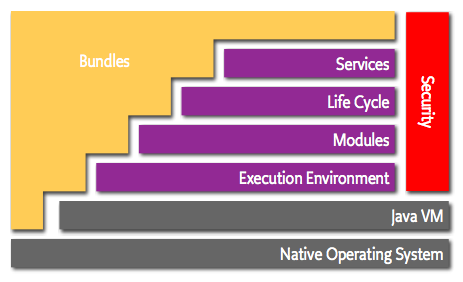
\includegraphics[width=10cm]{grafiken/osgi.png}
	\caption{OSGi Archetkur~\cite{osgiarch}}
	\label{osgiarch}
\end{figure}

Wie in Abbildung \ref{osgiarch} zu erkennen, ist die OSGi Service Plattform als
eine Schichtenarchitektur aufgebaut. Die Architektur setzt sich aus den
folgenden Schichten zusammen~\cite{osgiarch}:
\begin{itemize}
  \item \textbf{\em Bundles:} Bundles stellen die
  Modularisierungseinheit der OSGi Service Plattform dar. Diese
  k�nnen dynamisch in die Plattform installiert und gestartet, gestoppt und 
  deinstalliert werden, ohne dass die Plattform neugestartet oder angehalten 
  werden muss. 
  \item \textbf{\em Services:} Die Service-Schicht erlaubt das dynamische
  Verlinken verschiedener Bundles untereinander. Dies kann zum Austausch von
  Daten zwischen den Bundles oder zur Ausf�hrung von Funktionalit�ten genutzt werden.
  \item \textbf{\em Life Cycle:} Der Life Cycle k�mmert sich um das Bundle
  Management. Es k�nnen dar�ber Bundles installiert und gestartet, gestoppt und
  deinstalliert werden.
  \item \textbf{\em Modules:} Diese Schicht beschreibt, wie Code von Bundles
  exportiert und von anderen Bundles importiert werden kann. Dabei wird
  sichergestellt, dass nicht exportierter Code, nicht von anderen Bundles
  verwendet werden kann. Neben der Sicherstellung von Import und Export k�mmert
  sich diese Schicht auch um die Versionierung von freigegebenen Schnittstellen.
  So kann dieselbe Schnittstelle in unterschiedlichen Versionen parallel
  verwendet werden.
  \item \textbf{\em Security:} Die Security-Schicht k�mmert sich um das
  Rechtemanagement innerhalb der OSGi Service Plattform. So lassen sich
  Bundles soweit einschr�nken, dass bestimmte Aktionen erlaubt oder verboten
  sind. Diese Schicht geh�rt nicht zur Kernkomponenten der
  OSGi-Plattform und ist somit optional.
  \item \textbf{\em Execution Environment:} Diese Schicht spezifiziert die
  Mindestanforderungen an die Laufzeitumgebung, zur Ausf�hrung der OSGi
  Service Plattform.
\end{itemize}

\subsection{Verf�gbare OSGi Container f�r Android}
Dadurch das Android auf einer Teilmenge des Apache Harmony Projektes basiert,
deckt es einen Gro�teil der Standard Java
Klassenbibliothek~\cite{apacheharmony}. Dies erlaubt die Ausf�hrung von OSGi auf
Android. Die Ausf�hrungsumgebung der Bundles wird auch als OGSi Container
bezeichnet. Folgende OSGi Container sind unter Android lauff�hig.

\subsubsection{Apache Felix}
Apache Felix ist eine Open-Source-Implementierung des OSGi R4 Version 4.2
Standards~\cite{apachefelix}. Es ist der zurzeit einzige auf Android lauff�hig
freie OSGi Container. Leider bietet Apache Felix keine integration in das
Android System. Es l�sst sich zurzeit nur per Konsole starten und verwalten.
Dies macht es aufwendig Android Applikationen zu entwickeln die in Apache Felix
laufen~\cite{apachefelixandroid}.

\subsubsection{Dynamix Framework}
Das Dynamix Framework ist eine Open-Source Middleware um die Entwicklung von
kontextsensitiven Anwendungen auf Android Smartphones zu vereinfachen. Das
Framework l�uft im Hintergrund auf dem Android Smartphone. Durch die verwendung
von dynamisch installierten Plug-Ins, die durch die Dynamix Infrastruktur zur
Verf�gung gestellt werden, modelliert das Framework Kontextinformationen.
Kontextinformationen werden dabei durch die Sensorik oder andere externe Systeme
zur Verf�gung gestellt. Diese Informationen k�nnen dann anderen auf dem
Smartphone installierten Anwendungen in einer sicheren Art und Weise zur
Verf�gung gestellt werden.

Das Dynamix Framework basiert auf dem OSGi Container Apache Felix. Plug-Ins
werden dabei in Form von Bundles installiert. Das Framework k�mmert dabei um den
Lebenszyklus eines Plug-Ins und erlaubt das senden von Kontextinformationen an
registrierte Anwendungen. Der vom Dynamix Framework zur Verf�gung gestellt OSGi
Container bietet eine integration in das Android System. Er l�uft dabei als
Service im Hintergrund. Er erlaubt durch die sogenannte Context-Firewall, einen
durch den Anwender geregelten Zugriff, auf die von den Plug-Ins generierten
Kontextinformationen durch registrierte Anwendungen~\cite{dynamixframework}.

\section{Datenpersistierung mit Db4o}
db4o ist eine Objektdatenbank f�r die Java und .NET Plattform, die sich durch
ihre geringe Gr��e von nur 600KB f�r die Einbettung in Anwendungen eignet. Durch
ihre geringe Gr��e eignet sie sich auch f�r die Verwendung von mobilen Ger�ten
wie Smartphones, in diesem Fall Android. db4o bietet hierbei eine alternative zu
der in Android enthaltenden relationalen Datenbank SQLite. So ist db4o
schemafrei und erlaubt die Speicherung beliebig komplexer Objekte ohne die
Verwendung eines Objekt Relationalen Mappers (ORM). Die Datenspeicherung erfolgt
wie bei SQLite in einer Datei. db4o verwendet im Gegensatz zu relationalen
Datenbanken kein SQL, sondern Query By Example (QBE), Critera Queries sowie
Native Anfragen. Bei Query By Example wird anhand eines Beispiel Objektes nach
�hnlichen Objekten gesucht. Bei Critera Queries werden SQL Queries anhand von
entsprechenden Methodenaufrufen nachgebildet und bei Nativen Queries k�nnen
beliebig komplexe Suchanfragen in Java direkt implementiert werden.

	\chapterfin
	\chapter{Konzeption}
\label{cha:konzeption}
Im Folgenden wird auf die Konzeption der Anwendung eingegangen. Die Konzeption
umfasst die �berf�hrung der Anforderungen in ein Vorgehen, wie die Anforderungen
Softwareseitig realisiert werden k�nnen.

\section{Plug-In System}
Ein Erweiterungssystem oder wie hier benannt Plug-in System k�mmert sich um die
Verwaltung von Erweiterungen bzw. Plug-Ins. Das Plug-In System erlaubt die
Erweiterung der Anwendung auch nach ihrer Installation auf dem Smartphone. In
diesem Fall soll die Anwendung im nachhinein um Plug-Ins erweitert werden, die
Sensordaten sammeln.

Zur Realisierung eines Plug-Ins Systems auf Android gibt er zwei Ans�tze. Der
erste Umfasst die Verwendung eines bereits existierenden Plug-Ins Systems (z.B.
\acs{osgi}) oder die Entwicklung eines eigenen Plug-Ins Systems. Im Folgenden
sollen diese zwei Ans�tze genauer betrachtet werden.

\subsection{Evaluation der \acs{osgi} Plattform f�r Android}
Die Verwendung von \acs{osgi} als Modularisierung bzw. Plug-In System w�rde
folgenden Vorteile bieten:

\begin{itemize}
  \item Modularisierung und dynmaisches Laden von neuen Erweiterungen.
  \item Ausf�hrung von Erweiterungen in einer Art Sandbox. Damit ist gemeint,
  dass durch die Bereitstellung separater ClassLoader der Zugriff auf einzelne
  Elemente der Bibliothek verhindert werden kann.
  \item Versionierung von Plug-Ins.
\end{itemize}

Eine eigenst�ndige Integration von \acs{osgi} in Android war im Rahmen dieser
Masterarbeit aus zeitlichen Gr�nden nicht m�glich. Grund hierf�r ist die
abweichende Entwicklung von Anwendungen f�r Android und Java SE und die daraus
resultierende n�tige Anpassung von \acs{osgi} an Android. Dieser Aufwand war
zeitlich nur schwer absch�tzbar. Die Verwendung eines bereits f�r Android
optimierten Frameworks ist somit unumg�nglich. Als einziges freies Framework
steht zurzeit nur das Dynamix Framework zur Verf�gung. Eine Verwendung des
Dynamix Frameworks war aber zum Bearbeitungszeitpunkt dieser Arbeit leider nicht
m�glich. Dem Autor wurde in einem pers�nlichen Gespr�ch mit dem Dynamix
Entwickler Dr.-Ing. Darren Carlson von dessen Verwendung abgeraten. Der Grund
hierf�r war das Recht fr�he Stadium des Frameworks und die damit verbundene
m�gliche Fehleranf�lligkeit, sowie die fehlende Dokumentation. Die Entwicklung
eines eigenen Plug-Ins Systems war somit die einzige L�sung.

\subsection{Eigenentwicklung eines Plug-In Systems f�r Android}
\label{pluginsystemforandroid}
Bei der Entwicklung eines Plug-In Systems f�r Android gibt es zwei Ans�tze:

\begin{itemize}
  \item Man l�dt zur Laufzeit das Plug-In aus einem nachtr�glich
  heruntergeladenen \acf{jar}. Dies w�re der \acs{osgi} Ansatz.
  \item Man sieht ein Plug-In als Android Service an und kommuniziert mit diesem
  �ber {\em Intents} oder per \acs{ipc}.
\end{itemize}

Ersteres hat den Nachteil, dass eine Infrastruktur geschaffen werden m�sste, um
die Plug-Ins zur Verf�gung zu stellen. Letztes hat den Vorteil, dass ein Plug-In
als einfache Android Anwendung aus dem Android Market heruntergeladen und
installiert werden kann. Die Infrastruktur ist also schon vorhanden. Auch ist
letztes der Ansatz, der vom Android System am besten unterst�tzt wird.

Plug-Ins k�nnen somit als Service angesehen werden. Nach der Installation eines
Plug-Ins sollen sich neue Plug-Ins beim Plug-In System registrieren. Dazu soll
das Plug-In System nachdem es per Broadcast mitbekommen hat, dass ein neues
Plug-In installiert wurde, einen Broadcast an das neu installierte Plug-In
schicken. Das neue Plug-In soll daraufhin mit entsprechenden Plug-In
Informationen antworten. Folgende Informationen sollen bei der Anmeldung
�bermittelt werden:

\begin{itemize}
  \item Der {\bf Name} des Plug-Ins.
  \item Die {\bf Action} �ber die der Service per \acs{ipc} aufrufbar ist.
  \item Die {\bf Version} des Plug-Ins.
  \item Die {\bf URL} an die die gesammelten Daten �bertragen werden sollen.
  \item Die {\bf Periode} die angibt in welchen Zeitabst�nden Daten gesammelt
  werden sollen.
  \item Die maximale {\bf Ausf�hrungsdauer} des Plug-Ins, bevor es gestoppt
  wird.
  \item Eine Plug-In {\bf Beschreibung}.
  \item Das {\bf Interval} in dem die Daten regelm��ig �bertragen werden sollen.
  \item Eine Liste von {\bf Services} auf die das Plug-In zugreifen will.
  \item Eine Flag die angibt ob die {\bf gesammelten Daten nach der �bertragung
  gel�scht} werden sollen.
\end{itemize}

Hierbei ist anzumerken, dass Android nicht zwischen einem Plug-In und einer
anderen neu installierten Anwendung unterscheiden kann. Das Plug-In System
sendet somit an alle neu installierten Anwendungen eine Aufforderung zur
Registrierung. Dies ist aber kein Problem, da alle nicht Plug-Ins auf diese
Aufforderung nicht antworten werden.

Hat sich ein Plug-In erfolgreich registriert, werden die vom Plug-In
erhaltenden Informationen gespeichert und dem Benutzer in Form einer Plug-In
�bersicht pr�sentiert. Der Benutzer hat nun die M�glichkeit sich alle zuvor
beschriebenen Informationen anzuschauen. Dadurch soll er die M�glichkeit
erhalten zu entscheiden, ob ein Plug-In wirklich verwendet werden soll oder ob
der Benutzer dieses nicht will.

Ein Plug-In soll dabei bestimmte Zust�nde einnehmen k�nnen. Nach der
Installation soll ein Plug-In als neu dargestellt werden. Dies bedeutet der
Benutzer hat das Plug-In bisher nur installiert und noch keine weiteren
Einstellungen am Plug-In vorgenommen. Von diesem Zustand soll das Plug-In
aktiviert werden k�nnen. Das hei�t das Plug-In wird in der, bei der
Registrierung angebenen Periode ausgef�hrt. Soll ein Plug-In keine Daten mehr
sammeln, kann der Benutzer das Plug-In deaktivieren. Sollte ein aktiviertes
Plug-In nach einer bestimmten Zeit genug Daten gesammelt haben, soll es in den
Transferzustand �bergeben. Diese Zeit soll durch den Interval bei der Plug-In
Registierung angegeben werden. In diesem Zustand sollen die Daten f�r die
�bertragung aufbereitet und lokal gespeichert werden. Wann die Daten nun
entg�ltig �bertragen werden, kann der Benutzer selbst entscheiden. Siehe hierzu
den Abschnitt \ref{periodicallytransfer}. Sind die Daten aufbereitet und
gespeichert worden, geht das Plug-In wieder in den aktivierten Zustand �ber.
Dieser Lebenzyklus des Plug-Ins ist in Grafik \ref{states} dargestellt.

\begin{figure}[h!] 
	\centering
	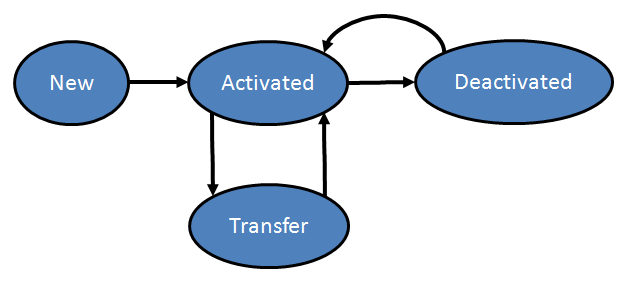
\includegraphics[width=10cm]{grafiken/states.png}
	\caption{Lebenszyklus eines Plug-Ins}
	\label{states}
\end{figure}

M�chte ein Benutzer ein Plug-In wieder entfernen, kann er dieses �ber den
Anwendungsmanager von Android machen. Der Benutzer soll aber auch direkt die
M�glichkeit besitzen, das Plug-In aus der �bersicht zu entfernen. Da es
sich beim Entfernen eines Plug-Ins um die deinstallation einer Androidanwendung
handelt, erh�lt das Plug-In System ebenfalls Broadcasts vom Android System. Dies
erlaubt dem Plug-In System die gespeicherten Daten vom Plug-In zu l�schen und
die Plug-In Informationen konsistent zu den anderen installierten Plug-Ins zu
halten.

\section{Transparentes Sammeln von personenbezogenen Daten}
Transparenz beim Sammeln von personenbezogenen Daten erh�lt man durch folgende
Voraussetzungen:

\begin{itemize}
  \item Der Benutzer muss immer die Kontrolle �ber ein Plug-In besitzen.
  \item Eine Manipulation bei der Darstellung der gesammelten personenbezogenen
  Daten darf nicht m�glich sein.
  \item Die Speicherung der Daten muss zentral in der Anwendung erfolgen, so das
  auch nur Daten �bertragen werden k�nnen die zentral gespeichert wurden.
  \item Bevor die Daten �bertragen werden, muss der Benutzer darauf hingewiesen
  werden, damit eine Kontrolle vor der �bertragung stattfinden kann.
\end{itemize}

Diese Vorsetzungen werden im folgenden genauer erl�utert.

\subsection{Sichere und kontrollierte Ausf�hrung von Plug-Ins}
\label{securepluginexecution}
Ein Plug-In wird dann sicher ausgef�hrt, wenn der Zugriff auf personenbezogene
Daten geregelt wird. Da der Zugriff auf diese Daten innerhalb von Android �ber
System Services geschieht, muss dieser Zugriff kontrolliert stattfinden. Es
sollte also geregelt werden, auf welche Services zugegriffen werden darf und
wenn ein Zugriff stattfindet, sollte dieser Zugriff protokolliert werden. Des
Weiteren sollte der Zugriff auf bestimmte Daten, die den Benutzer eindeutig
identifizieren (z.B. \acs{imsi}, Telefonnummer) komplett unterbunden werden. Aus
diesem Grund sollen dem Plug-In nicht die original Android System Services zur
Verf�gung gestellt werden, sondern stattdessen �berwachte bzw. sichere
Implementierungen der Android Services. Diese Services sollen jeden
Methodenzugriff protokolieren und zuvor beschriebene gef�hrliche Methoden gar
nicht erst anbieten.

Dabei sollen einem Plug-In nicht von vorne rein alle Services �bergeben werden,
sondern nur die, die in den Plug-In Informationen angegebenen wurden. Sollte ein
Plug-In trotzdem versuchen auf einen Android System Service zuzugreifen, soll dieses dem
Benutzer bei der Aktivierung angezeigt werden. Der unerlaubte Versuch, Zugriff
auf einen Android System Service zu erlangen, kann �ber die angeforderten
Rechte des Plug-Ins entnommen werden. Es muss also vor der Aktivierung eine
Kontrolle dieser stattfinden.

Das hierbei entwickelte Konzept erweitert die von Android zur verf�gunggestellte
Sandbox, um weitere �berwachungsmechanismen, um den Schaden der durch ein
Plug-In entstehen kann zu verringern. Der hierbei gr��te anzunehmende Schaden
ist die �bertragung von personenbezogenen Daten, ohne das Wissen und die
Erlaubnis des Benutzers.

\subsection{Einheitliche Pr�sentation von gesammelten Daten}
\label{unifiedrepresentation}
Um die von einem Plug-In gesammelten Daten pr�sentieren zu k�nnen, muss ein
entsprechendes Datenformat gew�hlt werden, an das sich alle Plug-Ins halten
m�ssen. Da die Struktur der Daten nicht bekannt ist, muss ein Datenformat
verwendet werden, dass unstrukturierte Daten abbilden kann. Ein solches
Datenformat wird in dem \acs{jsr}-170 beschrieben. Dieses \acs{jsr} beschreibt
die Speicherung von Daten im \acf{jcr}. Das dabei verwendete
Datenformat basiert auf sogenannten {\em Nodes} und {\em Properties} die sich zu
einer beliebigen hierarchischen Datenstruktur zusammensetzen lassen. Im Rahmen
dieser Masterarbeit soll eine eingeschr�nkte Implementierung des Standards
stattfinden, die Funktionalit�ten wie z.B. Versionierung und Locking nicht
ber�cksichtigt. Diese sind f�r die Erf�llung der Aufgabenstellung nicht n�tig.

Eine Node kann beliebige viele Kinder-{\em Nodes}, sowie {\em Properties}
besitzen. Ein Property besteht aus einem {\em Identifier} und einem {\em Value}.
Der {\em Value} selbst besteht dabei aus dem eigentlichen Wert der gespeichert
werden soll, sowie dem Typen des Wertes. Der Wert kann dabei vom Typ {\em
String}, {\em Date}, {\em Binary}, {\em Double}, {\em Decimal}, {\em Long} oder
{\em Boolean} sein. Nodes und Properties besitzen eine eindeutige ID, sowie ein
Modifizierungsdatum.

Zur Pr�sentation soll ein Viewer entwickelt werden, der die hierarchischen Daten
darstellen kann. Dabei soll jede Hierarchiestufe in Form einer Liste angezeigt
werden. Innerhalb der Liste werden alle Nodes und Properties gelistet. Klickt
man auf eine Node soll man in die n�chste Hierarchiestufe gelangen. �ber einen
Druck auf den hardwareseitigen Zur�ckbutton soll man eine Hierarchiestufe zur�ck
gelangen. Als Darstellungswert innerhalb der Liste soll bei einer Node das
Editierungsdatum und bei einer Property eine kombination aus dem {\em
identifier} und der Stringrepr�sentation des Wertes verwendet werden.

\subsection{Speicherung der Daten}
Die Speicherung der Daten soll zentral und in dem, in Abschnitt
\ref{unifiedrepresentation} beschriebenen Datenformat erfolgen. Durch die
zentrale und unmittelbare Speicherug der Daten als vereinheitlichte
Datenstruktur kann eine sofortige Pr�sentation der Daten geschehen, ohne die
Daten beim Plug-In selbst nachzufragen zu m�ssen. So m�ssen keine Daten vom
Plug-In selbst gespeichert werden, die Persistierung wird von der Anwendung
�bernommen. Die Speicherung der Daten soll per db4o erfolgen. db4o erlaubt dabei
die einfache Speicherung von komplexen hierarchischen Datenstrukturen, wie sie
im Abschnitt \ref{unifiedrepresentation} beschrieben ist.

Bei der Ausf�hrung eines Plug-Ins soll dieses vollen Zugriff auf die zuvor
gespeicherten Daten besitzen. Dadurch soll die M�glichkeit bestehen zuvor
gespeicherte Daten nachtr�glich zu bearbeiten und neue Datens�tze hinzuzuf�gen.

\subsection{Regelm��ige �bertragung der gesammelten Daten}
\label{periodicallytransfer}
Im Gegensatz zu anderen Anwendungen, in dem die Daten sofort ohne R�ckfrage des
Benutzers �bertragen werden, sollen sie in dieser Anwendung nur in regelm��igen
Abst�nden und nur nach Erlaubnis des Benutzers �bertragen werden. Die Abst�nde
sollen dabei durch das Plug-In definiert werden. Wird als �bertragungsinterval
z.B. ein Tag angegeben, so soll der Benutzer, wenn das Plug-In ein Tag lanbg
aktiv war, in den zuvor beschriebenen Transferzustand �bergehen. Sollte das
Plug-In in dieser Zeit deaktiviert worden sein, soll diese Zeit nicht in die
�bertragungszeit mit eingerechnet werden. Es wird nur die Zeit verwendet in der
das Plug-In aktiv war.

Befindet sich das Plug-In im Transferzustand, sollen die bis dahin vom Plug-In
gesammelten Daten gesichert und f�r die �bertragung vorbereitet werden. Das
Plug-In kann nun wieder aktiviert werden und weiter Daten sammeln. Der Benutzer
soll nun vor der �bertragung alle Aktivit�ten des Plug-Ins betrachten k�nnen.
Das bedeutet, alle Zugriffe auf die Services, sowie die vom Plug-In gesammelten
Daten.

Ist der Benutzer mit einer �bertragung der Daten einverstanden, kann er die
Daten zu einem beliebigen Zeitpunkt in der Zukunft �bertragen. Die Daten sollen
dabei an die, in den Plug-In Information enthaltenen URL �bertragen werden.
Sollte der Benutzer nicht mit der �bertragung der Daten einverstanden sein, so
soll er die M�glichkeit besitzen, die vom Plug-In gesammelten Daten zu
verwerfen. Da eine �bertragung zu einem beliebigen Zeitpunkt in der Zukunft
stattfinden kann, kann es passieren, dass sich mehre �bertragungen ansammeln
k�nnen. Diese �bertragungen sollen �bersichtlich aufgelistet werden.

Bei der �bertragung m�ssen neben den von dem Plug-In gesammelten Daten, auch
Informationen �ber das verwendete Plug-In und eine eindeutige Benutzerkennung
�bertragen werden. Dadurch kann auf der Serverseite eine eindeutige Zuordnung
zu einem Plug-In stattfinden, sowie zu einem Benutzer. Die Benutzerkennung soll
dabei anonymisiert sein. Hierzu mehr in Abschnitt \ref{anonymisation}.

\section{Serverseitiger Empfang und Verarbeitung der Daten}
Neben der reinen Android Anwendung soll auch eine Serverkomponente entwickelt
werden, die die vom Plug-In gesammelten Daten empfangen kann. Zum Empfang der
Daten auf dem Server soll auf bereits bekannte Standards wie \acs{http} und
\acs{json} gesetzt werden. Dazu soll auf dem Server ein \acs{rest}ful Webservice
zur Verf�gung gestellt werden, um die von der Anwendung in \acs{json} kodierten
Daten zu empfangen. \acs{json} erlaubt dabei, die �bertragung der Daten mit
einem sehr geringen Overhead.

Da die Daten von der Anwendung in dem zuvor beschriebenen sehr allgemeinen
Datenformat empfangen werden, ist eine Konvertierung der Daten in ein
spezifisches Datenformat vorzunehmen. Dadurch soll eine einfachere Speicherung
in relationale Datenbanken stattfinden k�nnen.

\section{Anonymisierung des Benutzers}
\label{anonymisation}
Wie bereits in Abschnitt \ref{anonym} beschrieben, sind die von der Anwendung
empfangenen Daten ohne eine eindeutige Benutzerkennung nicht �ber mehre
�bertragungen zu einem Benutzer zuordbar. Diese Zuordbarkeit ist aber
interessant, wenn man z.B. die Bewegungen von Personen �ber einen l�ngeren
Zeitraum �berwachen m�chte. Ohne eine Benutzerkennung w�re dies immer nur
innerhalb eines �bertragungsintervals m�glich. Um dieses Problem zu l�sen, ist
eine eindeutige Benutzerkennung n�tig, die bei jeder �bertragung mitgesendet
wird. Bei der Benutzerkennung ist auf folgendes zu achten:

\begin{itemize}
  \item Die Benutzerkennung darf auf keine reale Person �bertragen werden
  k�nnen.
  \item Die Benutzerkennung muss zwischen verschiedenen Plug-Ins unterschiedlich
  sein.
  \item Auch bei einem Wechsel des Ger�ts soll die selbe eindeutige
  Benutzerkennung ohne jeglichen Interaktion mit dem Benutzer generiert werden
  k�nnen.
\end{itemize}

Um eine eindeutigen Benutzerkennungen zu berechnen, m�ssen eindeutige Werte vom
Plug-In, sowie vom Benutzer verwendet werden. Da der Wert vom Benutzer ohne
Interaktion ermittelt werden soll, muss hier ein Wert verwendet werden, der
Benutzer spezifisch ist und sich bereits auf dem Smartphone befindet. Zu diesem
Zweck kann die \acs{imsi} verwendet werden. Diese Nummer identifiziert einen
Benutzer eindeutig im \acs{gsm} und \acs{umts} Netz. Als Plug-In Wert kann die
{\em Action} verwendet werden, die f�r jedes Plug-In eindeutig ist.

Aus der Kombination von Plug-In {\em Action}, sowie \acs{imsi} l�sst sich nun
ein eindeutiger Identifier berechnen. Zur Berechung eignen sich Hash-Funktionen.
Diese erlauben die Generierung von eindeutigen Werten und sind nur mit sehr
hohem Aufwand umkehrbar. Als Hash-Funktion soll eines aus der Gruppe der
\acs{sha}-2 Algorithmen verwendet werden, da diese das zurzeit sicherste
Verfahren sind. Die eindeutige Benutzerkennung kann nun durch die Kontatination
aus Plug-In Action und \acs{imsi} und der anschlie�enden Anwendung eines
\acs{sha}-2 Algorithmus berechnet werden. Die sich dabei ergebene
Benutzerkennung bietet maximale anonymit�t bei maximalen Komfort des Benutzers.
Diese Kennung soll nun bei jeder �bertragung mit �bertragen werden.

	\chapterfin
	\chapter{Realisierung}
\label{cha:realisierung}
In diesem Kapitel wird die aus dem Konzept entwickelte Realisierung beschrieben.
Die Anwendung tr�gt dabei den Arbeitstitel {\em Mobile Data Collector}, w�hrend
das Framework zur Erstellung von Plug-Ins den Namen {\em Mobile Data Collection
Framework} tr�gt.

Der {\em Mobile Data Collector} wird als Open Source Projekt entwickelt und kann
entweder von der beiliegenden CD oder von Github unter der Adresse
\url{https://github.com/mlegenhausen/mdcf} bezogen werden. Das Projekt ist dabei
in die folgenden Teile gegliedert:

\begin{itemize}
  \item {\bf MobileDataCollector}: Die {\em Mobile Data Collector} Android
  Anwendung.
  \item {\bf MobileDataCollectionFramework}: Das Framework zur Entwicklung von
  Plug-Ins.
  \item {\bf LocationTrackerPlugin}: Ein Beispiel Plug-In zum Sammeln von
  Standortdaten.
  \item {\bf NoiseTrackerPlugin}: Eine Erweiterung des {\em
  LoationTrackerPlugin}, bei dem neben der aktuellen Position, auch die
  Lautst�rke gespeichert wird.
  \item {\bf mdcf-remote}: Framework zur Entwicklung der Serverkomponente.
  \item {\bf mdcf-locationtracker-remote}: Eine Beispielserverkomponente f�r
  das {\em LocationTrackerPlugin}.
  \item {\bf mdcf-noisetracker-remote}: Eine Beispielserverkomponente f�r das
  {\em NoiseTrackerPlugin}.
\end{itemize}

\section{Architektur des Mobile Data Collection Frameworks}
Das {\em Mobile Data Collection Framework} dient zur Erstellung von Plug-Ins. Es
beinhaltet alle Klassen und Schnittstellen, die zwischen dem {\em Mobile Data
Collector} und dem Plug-In geteilt werden, um eine Kommunikation zwischen beiden
Komponenten zu erm�glichen. Das Framework wird als Android Bibliothek zur
Verf�gung gestellt.

Das Framework ist in drei Teile gegliedert. Zum einen Klassen und Interfaces,
die es einem Plug-In erlauben sich an dem Plug-In System anzumelden und mit
diesem zu kommunizieren. Zum anderen einer Implementierung der in Abschnitt
\ref{unifiedrepresentation} beschriebenen Datenstruktur sowie der in Abschnitt
\ref{securepluginexecution} beschriebenen sicheren Android Services.

Ein Plug-In wird dadurch definiert, dass es die {\em Plugin}-Schnittstelle
implementiert. Diese stellt alle f�r das Plug-In System n�tigen Methoden
zur Verf�gung, um mit dem Plug-In zu interagieren. Die Schnittstelle selbst
besteht aus einer Reihe von {\em Settern}, mit denen die sicheren Versionen der
Android System Services und der {\em PersistenceManager} gesetzt werden, sowie
einer {\em run}-Methode, mit der das Plug-In ausgef�hrt wird. Da die {\em
Setter}-Implementierungen trivial und in den meisten F�llen identisch sind, gibt
es zur Vereinfachung die Klasse {\em AbstractPlugin}. Erbt man von dieser
Klasse, muss nur noch eine vereinfachte Version der {\em run}-Methode, die {\em
onRun}-Methode implementiert werden.

Innerhalb der {\em run}- bzw. {\em onRun}-Methode kann auf die gesetzten
Services zugegriffen werden. Die Services bieten alle in der Android Dokumentation beschriebenen
Methoden. Neben den Services kann auch auf einen {\em PersistenceManager}
zugegriffen werden. Dieser erlaubt �ber die {\em getWorkspace}-Methode den
einfachen Zugriff auf alle bisher gespeicherten Daten. Die zur�ckgegebene
Datenstruktur kann dann innerhalb des Plug-Ins beliebig manipuliert werden.
Wurden alle Daten erfolgreich manipuliert, k�nnen die �nderungen mit der {\em
save}-Methode gespeichert werden.

Die Registrierung eines Plug-Ins erfolgt durch die Antwort auf den vom Plug-In
System versendeten {\em Broadcast}, der nach der Installation einer neuen
Anwendung versendet wird. Um auf diesen {\em Broadcast} zu antworten, muss ein
{\em Broadcast Receiver} implementiert werden. Zu diesem Zweck existiert bereits
eine Implementierung des {\em Broadcast Receiver}, der {\em
AbstractPluginRegister}. Erbt man von dieser Klasse, muss man die {\em
onRegister}-Methode implementieren. Diese muss ein {\em PluginInfo}-Objekt
zur�ckliefern, welche die Plug-In Informationen enth�lt. Bei dem {\em
PluginInfo}-Objekt handelt es sich um ein Java \acs{pojo}, dass die in Abschnitt
\ref{pluginsystemforandroid} beschriebenen Attribute besitzt. Neben der reinen
Java Konfiguration kann man das Objekt auch aus einer \acs{xml}-Datei generieren
lassen. Dazu muss man von der {\em XMLPluginRegister}-Klasse erben und den Pfad
zur Konfigurationsdatei als Konstruktorparameter �bergeben. Dabei muss darauf
geachtet werden, dass die Datei sich im {\em Java Classpath} befindet.

Damit das implementierte Plug-In und der {\em Broadcast Receiver} vom Android
System gefunden werden kann, m�ssen entsprechende Eintr�ge in der {\em
AndroidManifest.xml} erfolgen.

Konkrete Beispiele zur Implementierung und Konfiguration sind dem Kapitel
\ref{cha:leitfaden} zu entnehmen.

\section{Architektur des Mobile Data Collectors}
Die Architektur des {\em Mobile Data Collector} ist in Abbildung
\ref{architecture} dargestellt. Wie in der Abbildung zu erkennen, stellt der
{\em Plug-In Service} (blau) die zentrale Komponente des {\em Mobile Data
Collector} dar. Er beherbergt das gesamte Plug-In System und k�mmert sich somit
um die Verwaltung und Ausf�hrung von Plug-Ins. Er speichert alle von den
Plug-Ins gesammelten Daten in einer \acs{db4o}-Datenbank (gelb). Sollte ein
Plug-In auf die Android System Services (grau) zugreifen, geschieht dies, aus
Transparenzgr�nden, ebenfalls �ber den Plug-In Service.

\begin{figure}[h!] 
	\centering
	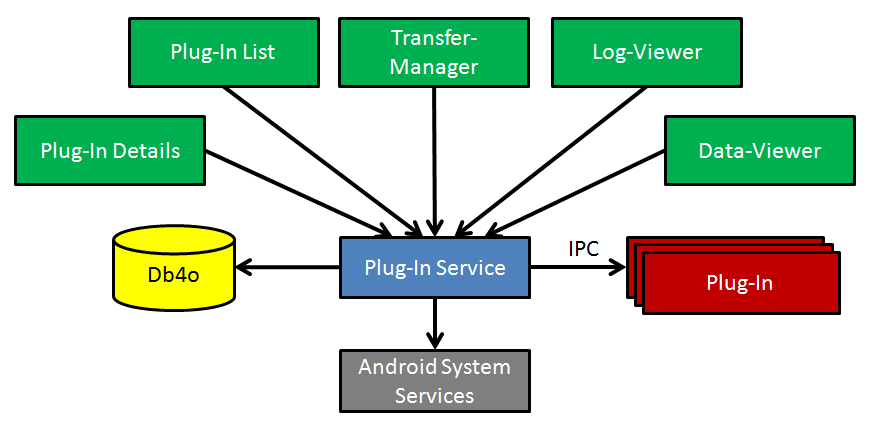
\includegraphics[width=13cm]{grafiken/architecture.png}
	\caption{Architektur des Mobile Data Collector}
	\label{architecture}
\end{figure}

F�r die Benutzerinteraktion mit dem Plug-In Service stehen eine
F�lle von {\em Activities} (gr�n) zur Verf�gung. Diese {\em Activities} sind:

\begin{itemize}
  \item Der {\bf Plug-In List} dient zur Auflistung von installierten Plug-Ins.
  \item Die {\bf Plug-In Details} erlaubt die Einsicht von Plug-In
  Informationen.
  \item Der {\bf Log-Viewer} dient zur Auflistung von Aufrufen von Android
  System Services.
  \item Der {\bf Data-Viewer} erlaubt die Betrachtung von allen vom Plug-In
  gesammelten Daten.
  \item Der {\bf Transfer-Manager} listet alle ausstehenden �bertragungen auf
  und erlaubt die nachtr�gliche Betrachtung aller bis zur �bertragung
  gesammelten Daten sowie deren Verwaltung.
\end{itemize}

Die Pfeile ausgehend vom und zum {\em Plug-In Service} stellen die
Aufrufrichtung dar. So ruft z.~B. der {\em Plug-In Service} immer die Plug-Ins
auf und die {\em Activities} den {\em Plug-In Service}.

Im Folgenden wird auf die zuvor beschriebenen Komponenten genauer eingegangen.

\subsection{Plug-In Service}
Der Plug-In Service stellt die zentrale Komponente zur Verwaltung von Plug-Ins
sowie deren Ausf�hrung dar. Er beinhaltet die gesamte Applikationslogik des
{\em Mobile Data Collectors}. Alle {\em Activities} greifen �ber eine
entsprechende Schnittstelle auf diesen Service zu. Der {\em Plug-In Service} l�uft
dabei dauerhaft im Hintergrund und f�hrt die Plug-Ins in den vorgegebenen
Abst�nden aus.

Neben der Service-Schnittstelle stellt das {\em PluginConfiguration}-Objekt eine
wichtige Datenstruktur dar. Alle zus�tzlichen Informationen �ber ein Plug-In,
die zur internen Verwaltung ben�tigt werden, werden im {\em
PluginConfiguration}-Objekt gespeichert. Dieses besitzt folgende Attribute:

\begin{itemize}
  \item {\bf Mode} gibt an, ob sich das Plug-In im {\em New}, {\em
  Activated}, {\em Deactivated} oder {\em Transfer} Zustand befindet. Im Letzteren
  werden die bisher gesammelten Daten f�r die �bertragung vorbereitet.
  \item {\bf State} gibt an ob, das Plug-In sich im {\em Resolved}, {\em
  Waiting} oder {\em Running} Zustand befindet. Im {\em Resolved} Zustand
  befindet es sich immer dann, wenn der {\em Mode} {\em New}, {\em Deactivated}
  oder {\em Transfer} ist. Zwischen den Zust�nden {\em Waiting} und {\em Running}
  wechselt das Plug-In, wenn es sich im {\em Mode} {\em Activated} befindet.
  \item {\bf Last Executed} gibt an, wann das Plug-In das letzte Mal ausgef�hrt
  wurde.
  \item {\bf Last Activated} gibt an, wann das Plug-In das letzte Mal aktiviert
  wurde.
  \item {\bf Total Activation Time} gibt summiert an wielange das Plug-In
  aktiviert war.
  \item {\bf Permissions} gibt an, welche Zugriffsrechte das Plug-In vom Android
  Betriebssystem ben�tigt. Im besten Fall ist dieses Attribut leer, da
  dies bedeutet, dass das Plug-In nicht auf reglementierte Ressourcen zugreifen
  muss.
  \item {\bf Log Records} protokolliert alle Zugriffe, die auf die sicheren
  Versionen der Android System Services stattgefunden haben.
  \item {\bf Transfers} beinhaltet eine Liste von ausstehenden �bertragungen.
  \item {\bf Workspace} beinhaltet alle vom Plug-In gesammelten Daten. Dabei
  handelt es sich um ein {\em Node}-Objekt, an dem alle zus�tzlichen Daten
  angehangen werden k�nnen.
\end{itemize}

Da die {\em PluginConfiguration} alle relevanten Plug-In Informationen, {\em
Log Records} und alle gesammelten Daten enth�lt, wird diese Datenstruktur 
zur Persistierung verwendet innerhalb der {\em db4o}-Datenbank.

\subsubsection{Service-Interface Definition}
Das Service-Interface beinhaltet die folgenden zentralen Methoden:

\begin{lstlisting}[language=java]
void addListener(PluginListener listener)
\end{lstlisting}

Erlaubt das Hinzuf�gen von {\em PluginListener}, die aufgerufen werden, wenn ein
neues Plug-In installiert bzw. entfernt wurde oder das Plug-In seinen {\em
Mode} oder {\em State} ge�ndert hat.

\begin{lstlisting}[language=java]
void addListener(TransferListener listener)
\end{lstlisting}

Erlaubt das Hinzuf�gen von {\em TransferListener}, die aufgerufen werden, wenn
eine neue �bertragung erstellt bzw. entfernt wurde.

\begin{lstlisting}[language=java]
void activate(PluginConfiguration configuration)
\end{lstlisting}

Aktiviert das mit der �bergebenen {\em PluginConfiguration} assoziierte Plug-In.

\begin{lstlisting}[language=java]
void deactivate(PluginConfiguration configuration)
\end{lstlisting}

Deaktiviert das mit der �bergebenen {\em PluginConfiguration} assoziierte
Plug-In.

\begin{lstlisting}[language=java]
PluginConfiguration getPluginConfiguration(PluginInfo info)
\end{lstlisting}

Liefert die zur {\em PluginInfo} dazu geh�rige {\em PluginConfiguration} zur�ck.
Existiert keine dazugeh�rige {\em PluginConfiguration}, so wird {\em null}
zur�ckgegeben.

\begin{lstlisting}[language=java]
List<PluginConfiguration> getPluginConfigurations()
\end{lstlisting}

Liefert alle installierten Plug-Ins zur�ck in Form von {\em
PluginConfiguration}-Objekten.

\begin{lstlisting}[language=java]
List<Transfer> getTransfers()
\end{lstlisting}

Liefert alle noch ausstehenden �bertragungen zur�ck. Sollten keine �bertragungen
vorhanden sein, wird eine leere Liste zur�ckgegeben.

\begin{lstlisting}[language=java]
void removeTransfer(Transfer transfer)
\end{lstlisting}

Entfernt den �bergebenen Transfer. Diese Methode sollte normal nur dann
aufgerufen werden, wenn das {\em Transfer}-Objekt auch an einen externen Server
�bertragen wurde.

\subsubsection{Plug-In Registierung}
Der Vorgang der Plug-In Registrierung ist in Abbildung \ref{register}
dargestellt.

\begin{figure}[h!] 
	\centering
	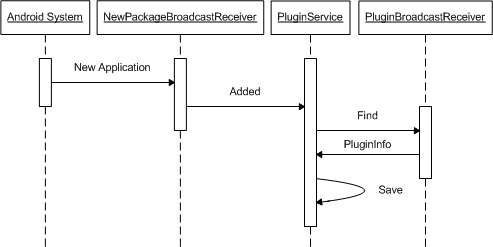
\includegraphics[width=13cm]{grafiken/register.png}
	\caption{Plug-In Registierung}
	\label{register}
\end{figure}

Wie in dem Sequenzdiagramm zu erkennen, sendet als Erstes das Android System
einen {\em Broadcast} mit dem Inhalt, dass eine neue Anwendung installiert
wurde. Dieser wird vom {\em PackageAddedBroadcastReceiver} empfangen. Daraufhin
versendet dieser ein {\em Added-Intent} an den Plug-In Service, dass eine neue
Anwendung installiert wurde. Dieser {\em Intent} wird von der {\em
onStartCommand}-Methode des Services empfangen. Der Plug-In Service versendet
daraufhin ein {\em Find-Intent} an die neu installierte Anwendung. Antwortet die
Anwendung nicht, so handelt es sich nicht um ein Plug-In. Antwortet die
neu installierte Anwendung mit einem {\em PluginInfo}-Objekt, so handelt es sich
um ein neues Plug-In.  Das vom Plug-In System empfangene {\em PluginInfo}-Objekt
wird nun vom Plug-In Service in einem {\em PluginConfiguration}-Objekt
gespeichert. Das Plug-In gilt nun als registriert. Die weitere Verwaltung
des Plug-Ins findet �ber das {\em PluginConfiguration}-Objekt statt.

\subsubsection{Plug-In Ausf�hrung}
Die Ausf�hrung des Plug-Ins findet im {\em PluginTaskManager} statt. Diese
Klasse verwaltet alle aktivierten Plug-Ins und f�hrt diese in dem vom Plug-In
vorgegeben Abstand aus. Dazu verwendet der {\em PluginTaskManager} einen
Thread-Pool, mit dem er eine bestimmte Anzahl von Plug-Ins parallel ausf�hren
kann. Zurzeit besitzt der Thread-Pool eine statische Gr��e von 1. Als
Thread-Pool Implementierung wurde der {\em ScheduledExecutorService} von der
Java Concurrency Bibliothek verwendet.

Wurde ein Plug-In aktiviert, wird dessen {\em PluginConfiguration}-Objekt an den
{\em PluginTaskManager} �bergeben. Dieser kapselt das {\em
PluginConfiguration}-Objekt zu einem {\em PluginTask}-Objekt. Beim {\em
PluginTask} handelt es sich um ein ausf�hrbares Objekt, dass das {\em
Runnable}-Interface implementiert. Dieser Task wird nun an den zuvor erw�hnten
Thread-Pool zur sofortigen Ausf�hrung �bergeben. Bei der Ausf�hrung wird aus der
{\em PluginInfo} die {\em Action} ausgelesen. Mit dieser ist es m�glich, die
Service-Schnittstelle des Plug-Ins aufzurufen. Konnte eine Verbindung zum
Plug-In hergestellt werden, werden zuerst alle f�r die Ausf�hrung n�tigen
Objekte gesetzt, um daraufhin das Plug-In auszuf�hren. Das Plug-In wird dabei
nur maximal f�r die im {\em PluginInfo} angegebene Zeit ausgef�hrt. Sollte diese
Zeit �berschritten werden, so wird das Plug-In vom Android System terminiert.
Nach der Ausf�hrung wird das Plug-In wieder zum Thread-Pool hinzugef�gt, um ihn
aber diesmal erst nach dem vom Plug-In definierten Abstand auszuf�hren. Dies
wiederholt sich solange, bis das Plug-In deaktiviert wurde oder eine �bertragung
vorbereitet wird. Dadurch, dass das Plug-In immer im Nachhinein wieder zum
Thread-Pool hinzugef�gt und nicht automatisch periodisch ausgef�hrt wird, wird
eine �berlappung der Plug-In Ausf�hrungen verhindert.

\subsection{Plug-In List}
Die Plug-In List dient zur Auflistung aller installierten Plug-Ins. Sind keine
Plug-Ins installiert, wird wie in Abbildung \ref{pluginlist} zu sehen, der
Benutzer daraufhin gewiesen.

\begin{figure}[h!] \centering
	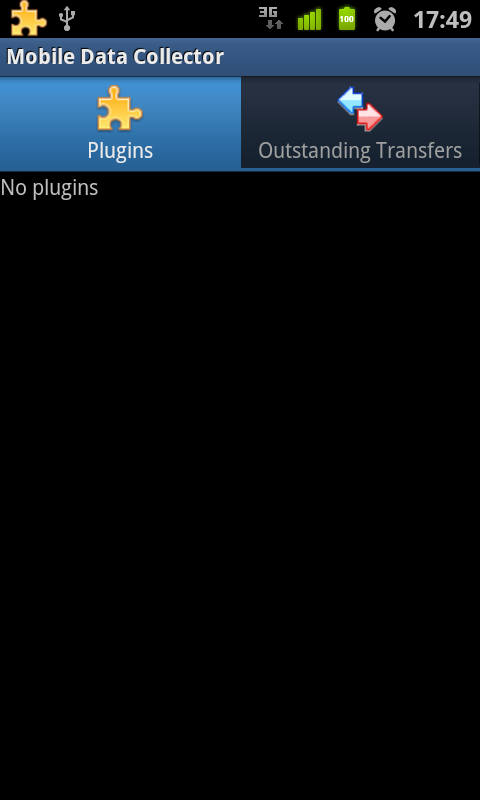
\includegraphics[width=5cm]{grafiken/pluginlist.png}
	\caption{Plug-In Viewer}
	\label{pluginlist}
\end{figure}

Neue Plug-Ins k�nnen �ber Eclipse, dem Android Market oder von der SD-Card
installiert werden. Um den Android Market schneller zu erreichen, kann auf
diesen wie in Abbildung \ref{more_plugins} �ber die Men�taste direkt zugegriffen
werden.

\begin{figure}[h!] \centering
	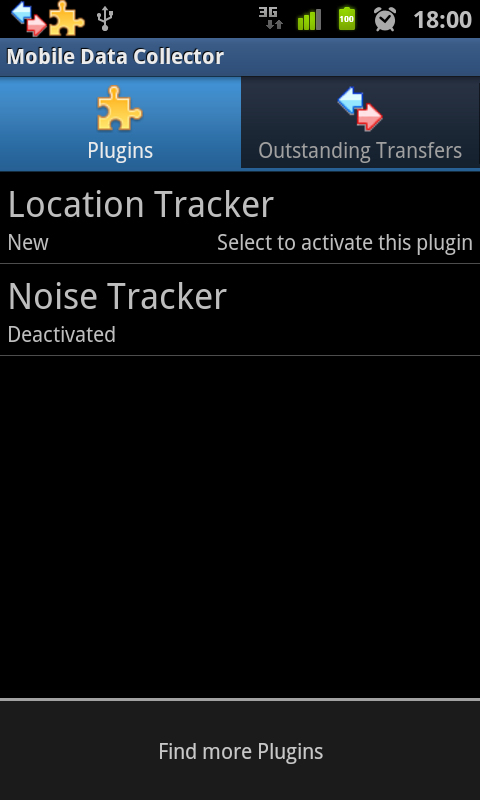
\includegraphics[width=5cm]{grafiken/more_plugins.png}
	\caption{Neue Plug-Ins installieren}
	\label{more_plugins}
\end{figure}

Wurden neue Plug-Ins installiert, werden diese wie in Abbildung \ref{plugins}
dargestellt im Plug-In Viewer angezeigt. Die installierten Plug-Ins befinden
sich zurzeit im Zustand {\em New}.

\begin{figure}[h!] \centering
	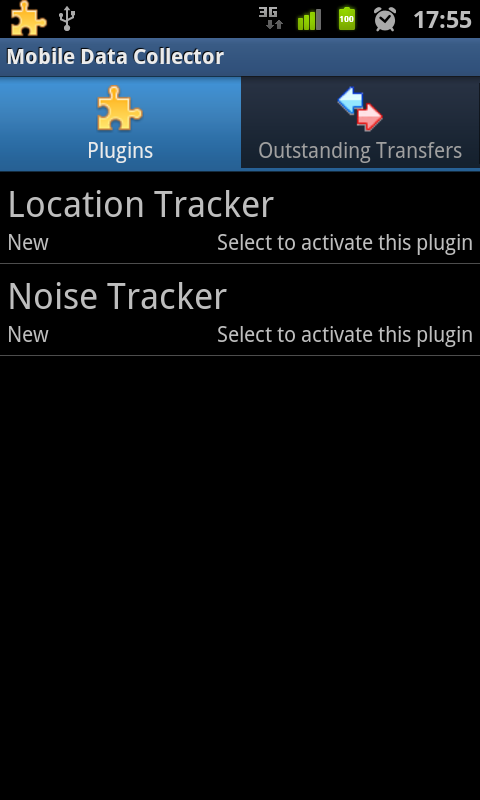
\includegraphics[width=5cm]{grafiken/plugins.png}
	\caption{Installierte Plug-Ins}
	\label{plugins}
\end{figure}

Durch das Anw�hlen eines Plug-Ins kann man dieses aktivieren. Bevor das Plug-In
aktiviert wird, werden wie in Abbildung \ref{activation} zu sehen, die Plug-In
Informationen angezeigt. Hat man alle Informationen kontrolliert und ist mit
diesen einverstanden, kann man durch das Dr�cken der {\em Activate} Schaltfl�che
das Plug-In aktivieren. Durch das Dr�cken von {\em Cancel} kann man den
Aktivierungsprozess abbrechen.

\begin{figure}[h!] 
	\centering
	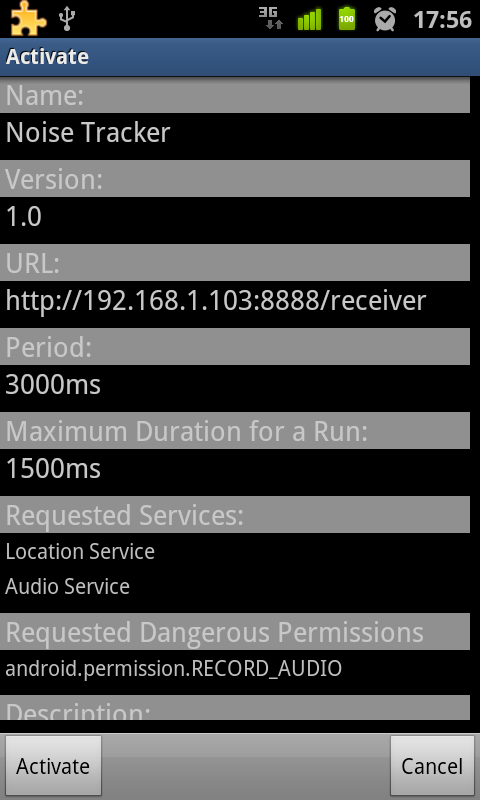
\includegraphics[width=5cm]{grafiken/activation.png}
	\caption{Plug-In aktivierung}
	\label{activation}
\end{figure}

Hierbei ist besonders auf die sogenannten {\em Dangerous Permissions} zu achten.
Diese weisen den Benutzer daraufhin, dass das Plug-In auf Rechte zugreifen
m�chte, die es normalerweise nicht braucht bzw. �ber diese, auf personenbezogene
Daten zugreifen k�nnte. Vor der Aktivierung wird deswegen der Benutzer durch die
in Abbildung \ref{activation_warning} dargestellte Warnung dar�ber informiert.

\begin{figure}[h!] 
	\centering
	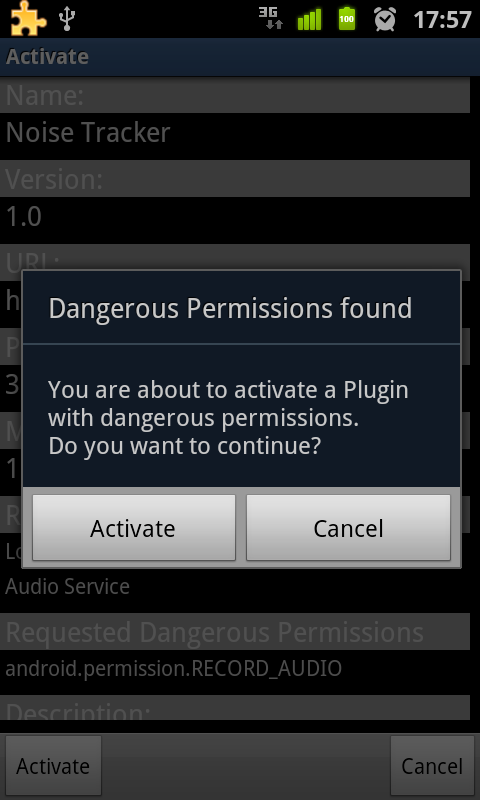
\includegraphics[width=5cm]{grafiken/activation_warning.png}
	\caption{Plug-In Aktivierung}
	\label{activation_warning}
\end{figure}

Ist sich der Benutzer trotzdem dar�ber bewusst, dass das Plug-In m�glicherweise
gef�hrlich sein k�nnte, so kann er durch das Dr�cken der {\em OK} Schaltfl�che
das Plug-In trotzdem aktivieren. Durch die {\em Cancel} Schaltfl�che kann die
Aktivierung abgebrochen werden.

Nach der Aktivierung eines Plug-Ins, wechselt die Anzeige von {\em
New} zu {\em Activated}. Siehe Abbildung \ref{activate}, indem das
{\em Noise Tracker} Plug-In aktiviert wurde. Die Anzeige f�r Datum und
Uhrzeit zeigt an, wann das Plug-In zum letzten Mal ausgef�hrt wurde.

\begin{figure}[h!] 
	\centering
	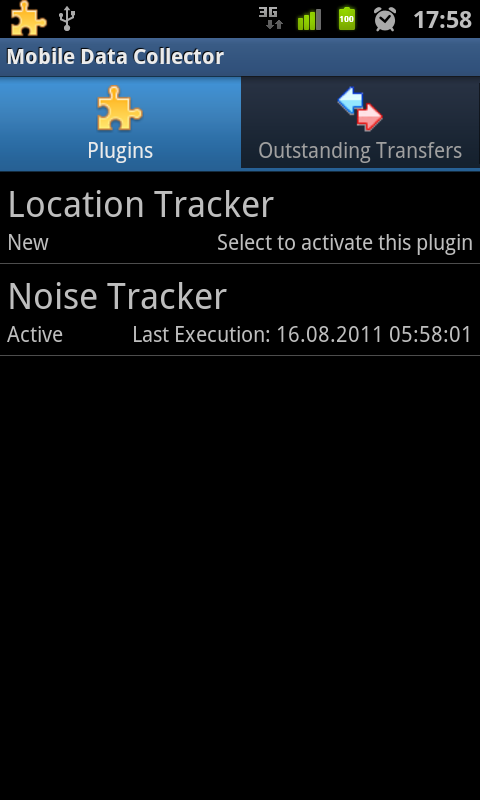
\includegraphics[width=5cm]{grafiken/active.png}
	\caption{Aktiviertes Plug-In}
	\label{activate}
\end{figure}

W�hlt man ein aktiviertes Plug-In erneut an, deaktiviert man dieses, wie in
Abbildung \ref{deactivated} zu sehen.

\begin{figure}[h!] 
	\centering
	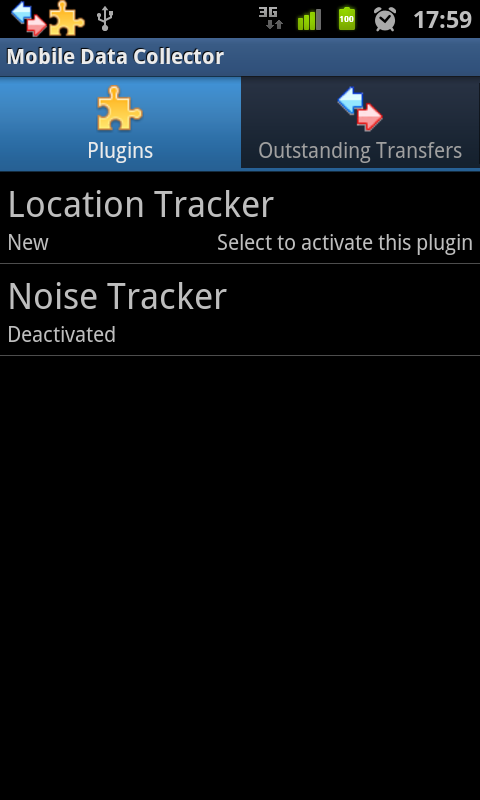
\includegraphics[width=5cm]{grafiken/deactivated.png}
	\caption{Deaktiviertes Plug-In}
	\label{deactivated}
\end{figure}

W�hlt man ein Plug-In durch ein langes Dr�cken aus, wird wie in Abbildung
\ref{plugin_context_menu} dargestellt, das Kontextmen� angezeigt. Dieses
erlaubt das Aktivieren und Deaktivieren eines Plug-Ins, das Anzeigen der Plug-In
Details (siehe hierzu Abschnitt \ref{plugin_details}), sowie das Deinstallieren
eines Plug-Ins.

\begin{figure}[h!] 
	\centering
	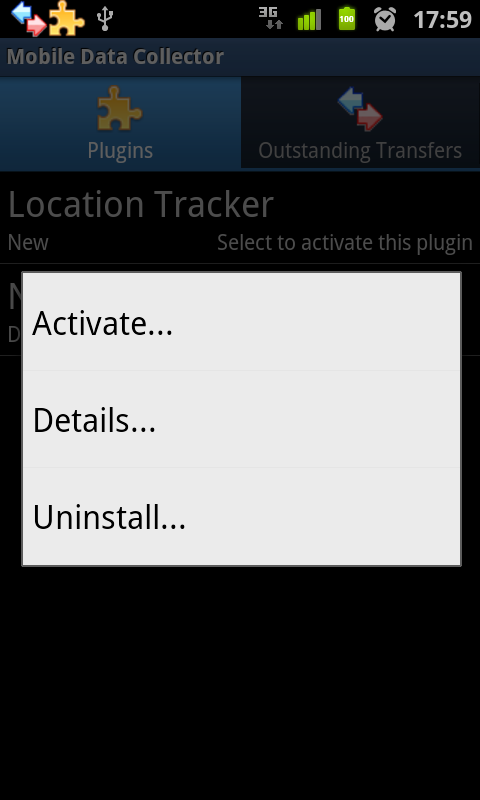
\includegraphics[width=5cm]{grafiken/plugin_context_menu.png}
	\caption{Context-Men� eines Plug-Ins}
	\label{plugin_context_menu}
\end{figure}

\subsection{Plug-In Details}
\label{plugin_details}
Der Benutzer hat �ber die {\em Plug-In Details} die M�glichkeit, zu jedem
Zeitpunkt, alle Informationen und Aktivit�ten eines Plug-Ins einzusehen. Die
{\em Plug-In Details} sind, wie im vorigen Abschnitt beschrieben, �ber das
Kontextmen� des Plug-Ins zu erreichen. �ffnet man die Details zu einem Plug-In,
werden die Plug-In Informationen, wie in Abbildung \ref{details}, angezeigt.
�ber die Tabs im oberen Bildschirmbereich gelangt man zu den weiteren Bereichen
{\em Logs} und {\em Collected Data}, die in den folgenden Abschnitten {\em
Log-Viewer} und {\em Data-Viewer} genauer erl�utert werden.

\begin{figure}[h!] 
	\centering
	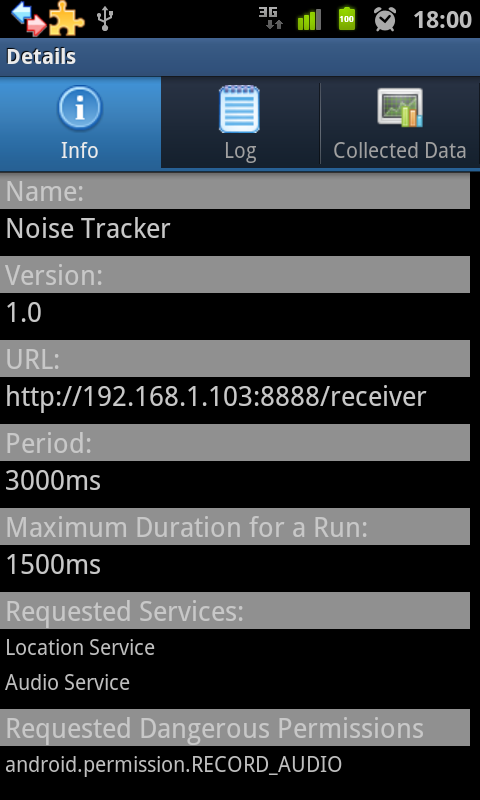
\includegraphics[width=5cm]{grafiken/details.png}
	\caption{Context-Men� eines Plug-Ins}
	\label{details}
\end{figure}

\subsubsection{Log-Viewer}
Der Log-Viewer dient zur Anzeige aller protokollierten Aktivit�ten eines
Plug-Ins. Mit Aktivit�ten ist der Zugriff auf die sicheren Android System Services gemeint.
Greift ein Plug-In auf eine Methode der Services zu, so wird ein Log-Eintrag
erstellt. Dieser enth�lt in benutzerverst�ndlicher Sprache, welche Informationen
abgefragt wurden. Ein Beispiel ist in Abbildung \ref{log} dargestellt.

\begin{figure}[h!] 
	\centering
	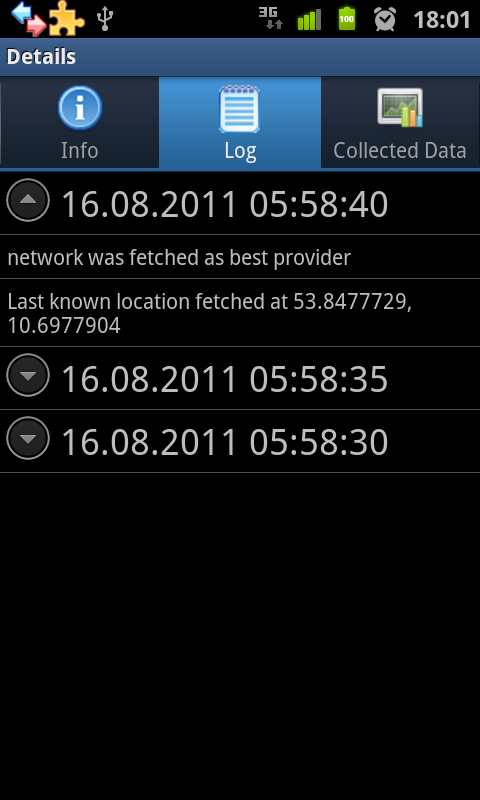
\includegraphics[width=5cm]{grafiken/log.png}
	\caption{Plug-In Logs}
	\label{log}
\end{figure}

Der Log ist dabei wie folgt aufgebaut. Jede Zeile zeigt an, wann das Plug-In
ausgef�hrt wurde. Durch die Auswahl eines Eintrags erweitern sich die Eintr�ge
um die eigentlichen Log-Eintr�ge. In diesem Fall sagen die Log-Eintr�ge aus,
dass am 16.08.2011 um 5:58:40 Uhr das Plug-In ausgef�hrt wurde. W�hrend dieser
Ausf�hrung wurde zur Lokalisierung des Benutzers das GSM/UMTS Netz ({\em
network}) verwendet und als Position wurden die Koordinaten am 53.8477729
L�ngengrad und am 10.6977904 Breitengrad ermittelt.

\subsubsection{Data-Viewer}
Der Data-Viewer dient zur Anzeige aller vom Plug-In gesammelten Daten bzw. aller
Daten, die das Plug-In sp�ter �bertragen m�chte. Einem Plug-In steht es frei,
beliebig viele private Daten f�r interne Zwecke zu sammeln.

Die im Konzept beschriebene hierarchische Datenstruktur l�sst sich durch den
Data-Viewer anzeigen. Dabei wird jede Ebene der Datenstruktur als Liste
dargestellt. In Abbildung \ref{collected_data_overview} wird die erste Ebene
angezeigt. Jeder anklickbare Knoten wird dabei als Datum angezeigt. Dieses
Datum gibt an, wann der entsprechende Datensatz das letzte Mal modifiziert
wurde. In diesem Fall werden drei Eintr�ge dargestellt. In diesem Beispiel
�berschneiden sich die Daten mit denen die im Log stehen. Damit ist gemeint,
dass nach jedem Zugriff auf den {\em LocationManager}, ein neuer Eintrag zu
den gesammelten Daten hinzugef�gt wurde.

\begin{figure}[h!] 
	\centering
	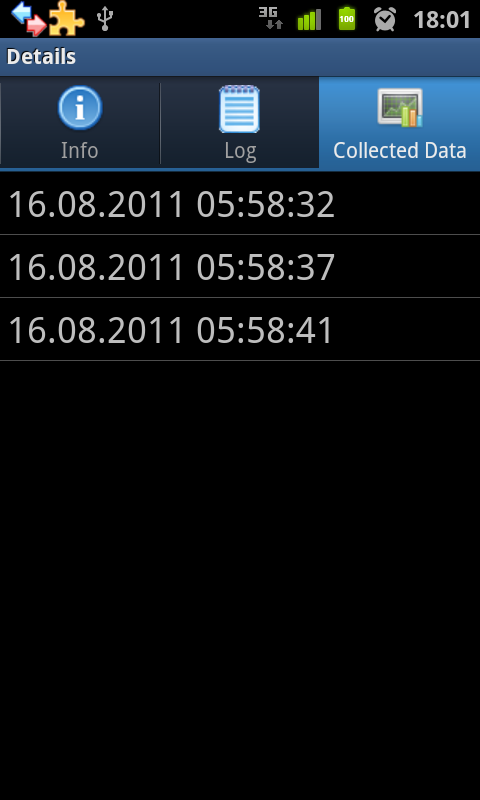
\includegraphics[width=5cm]{grafiken/collected_data_overview.png}
	\caption{Collected Data}
	\label{collected_data_overview}
\end{figure}

W�hlt man einen Knoten aus, so gelangt man in der Hierarchie eine
Ebene tiefer. Die unterhalb eines Knoten gespeicherten Daten k�nnen wie in
Abbildung \ref{collected_data_details} aussehen. In diesem Beispiel befinden sich auf
der angezeigten Ebene nur Eigenschaften. Diese Eigenschaften beschreiben von
oben nach unten die H�he, Geschwindigkeit, Lautst�rke, L�ngengrad, Genauigkeit,
Breitengrad, Drehrichtung und die Art der Positionsbestimmung. Um wieder auf
eine h�here Ebene zu gelangen, kann die Zur�cktaste verwendet werden.

\begin{figure}[h!] 
	\centering
	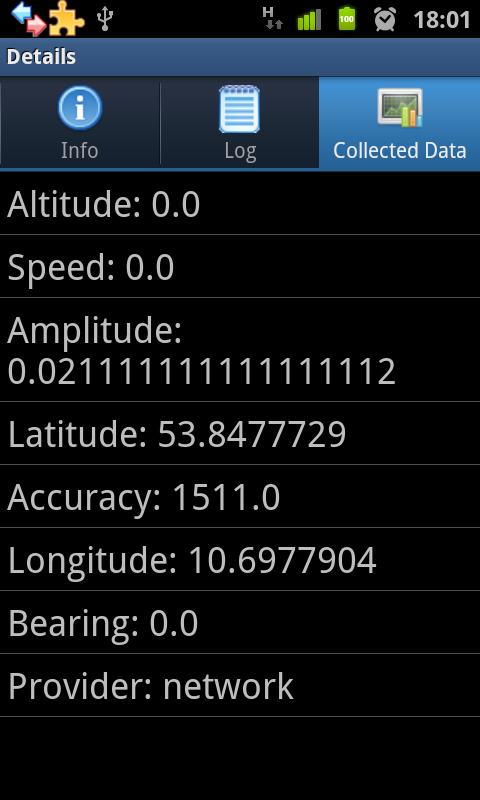
\includegraphics[width=5cm]{grafiken/collected_data_details.png}
	\caption{Gesammelte Daten eines Plug-Ins}
	\label{collected_data_details}
\end{figure}

\subsection{Transfer-Manager}
Der Transfer-Manager dient zur Verwaltung aller ausstehenden �bertragungen.
Sollte eine neue �bertragung ausstehen, so wird der Benutzer wie in Abbildung
\ref{new_transfer} dar�ber informiert.

\begin{figure}[h!] 
	\centering
	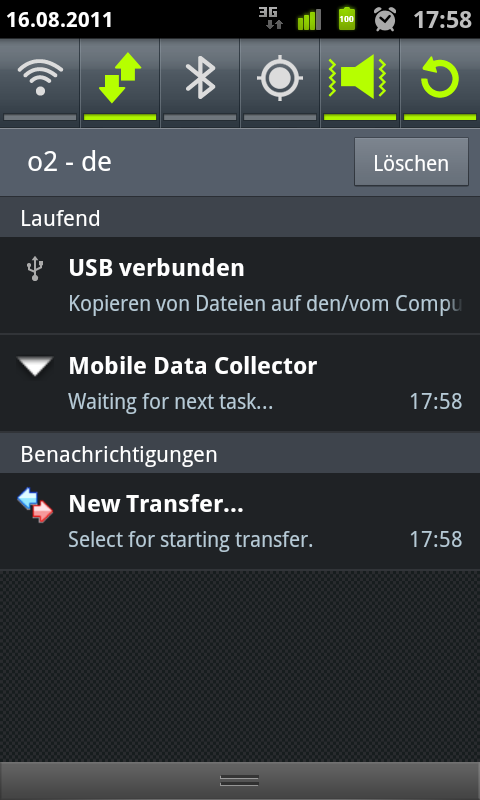
\includegraphics[width=5cm]{grafiken/new_transfer.png}
	\caption{Neue �bertragung}
	\label{new_transfer}
\end{figure}

Durch die Auswahl eines Eintrages gelangt der Benutzer in den
�bertragungsbereich des {\em Mobile Data Collectors}. Dieser kann bei einer
ausstehenden �bertragung wie in Abbildung \ref{transfer_pending} aussehen.

\begin{figure}[h!] 
	\centering
	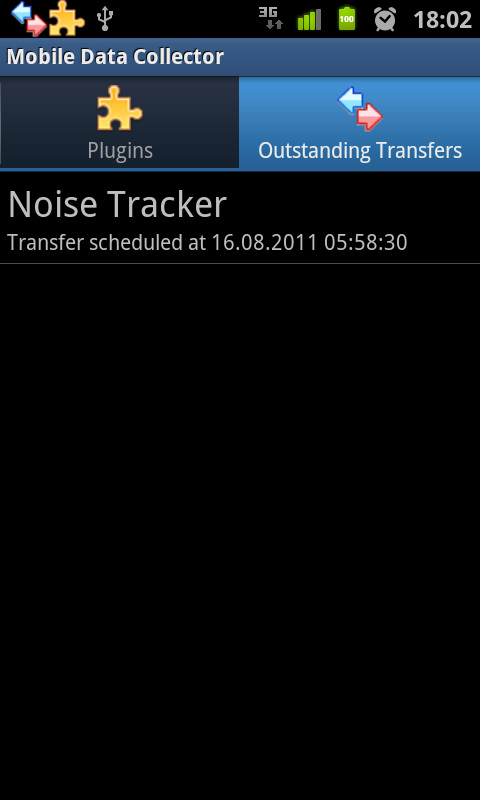
\includegraphics[width=5cm]{grafiken/transfer_pending.png}
	\caption{Ausstehende �bertragung}
	\label{transfer_pending}
\end{figure}

W�hlt der Benutzer den entsprechenden Eintrag aus, so gelangt dieser in die, in
Abbildung \ref{transfer_details} dargestellte, Detailansicht der �bertragung. In
dieser kann der Benutzer noch mal alle Informationen und Aktivit�ten des
Plug-Ins betrachten. Hierbei handelt es sich um einen Schnappschuss des aktuellen
Zustandes des Plug-Ins, den es hatte, als die �bertragung vorbereitet wurde.

\begin{figure}[h!] 
	\centering
	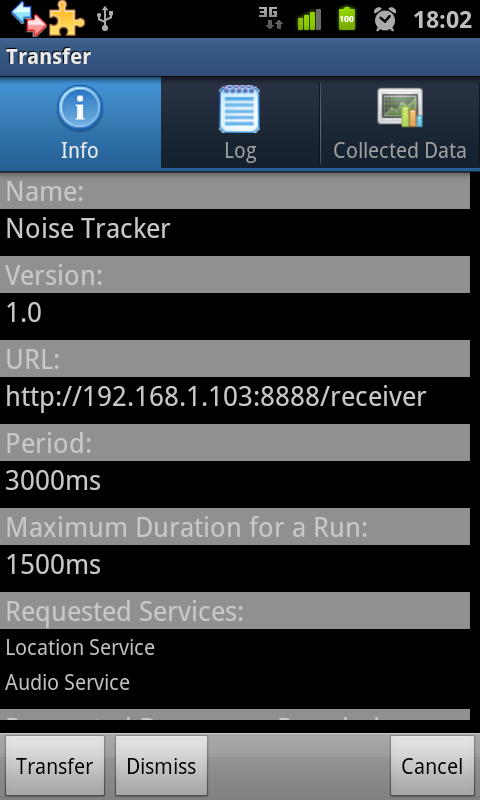
\includegraphics[width=5cm]{grafiken/transfer_details.png}
	\caption{�bertragungsdetails}
	\label{transfer_details}
\end{figure}

Hat der Benutzer alle Daten gesichtet und ist mit der �bertragung einverstanden,
kann er durch das Dr�cken der {\em Transfer} Schaltfl�che die �bertragung
einleiten. Daraufhin wird dem Benutzer der Fortschritt der �bertragung, wie in
Abbildung \ref{transfer_details_sending} und \ref{transfer_sending_notification}
zu sehen, als Dialog und Mitteilung angezeigt.

\begin{figure}[h!] 
	\centering
	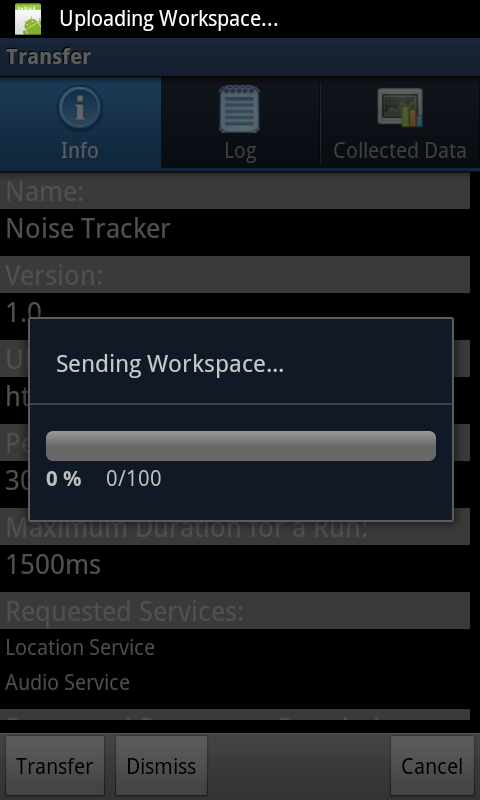
\includegraphics[width=5cm]{grafiken/transfer_details_sending.png}
	\caption{�bertragungsfortschritssdialog}
	\label{transfer_details_sending}
\end{figure}

\begin{figure}[h!] 
	\centering
	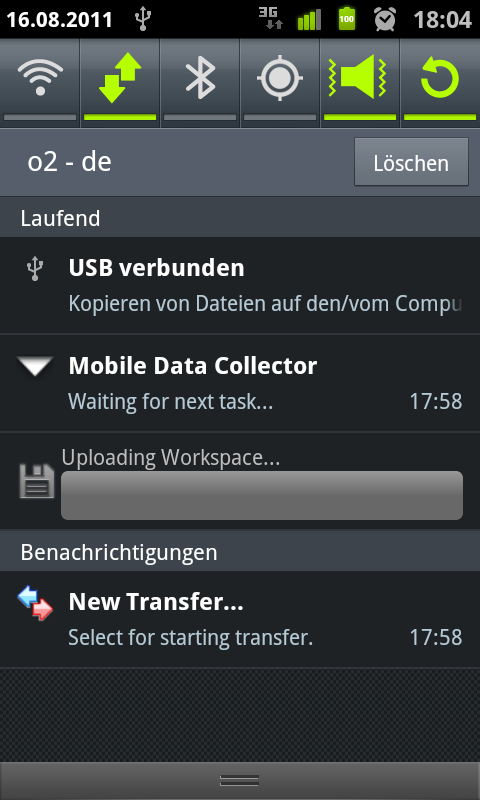
\includegraphics[width=5cm]{grafiken/transfer_sending_notification.png}
	\caption{�bertragungsfortschritt im Mitteilungsbereich}
	\label{transfer_sending_notification}
\end{figure}

Ist der Benutzer nicht mit der �bertragung seiner Daten einverstanden, kann er
durch die {\em Dismiss} Schaltfl�che, die �bertragung l�schen. Alle in der
�bertragung angezeigt Daten gehen daraufhin unwiderruflich verloren.

Intern wird bei der �bertragung zu einem Server eine \acs{http}-Verbindung
aufgebaut. Das Verbindungsziel wird hierbei dem \acs{url}-Attribut der Plug-In
Informationen entnommen. Die Daten, die in Form von Java-Objekten vorliegen, werden dann
mithilfe der GSON-Bibliothek in ein \acs{json}-Objekt �bersetzt~\cite{gson}. Da
sich dabei nur um eine Zeichenkette handelt, kann dieser einfach per \acs{http} versendet
werden.

\section{Aufbau der Serverkomponente}
Durch die Serverkomponente soll ein Plug-In Entwickler die M�glichkeit erhalten,
sehr schnell und einfach einen eigenen Server zu implementieren, um Daten von
einem Plug-In zu empfangen und zu verarbeiten. Die Serverkomponente steht als
Java-Bibliothek bereit und soll die einfache Integration in bestehende
Applikationsserver erlauben.

Die Serverkomponente ist wie folgt aufgebaut. Das {\em
TransferRequestReceiver}-Servlet empf�ngt die vom {\em Mobile Data Collector}
versandte \acs{json}-Datenstruktur und konvertiert diese in eine �quivalente
Java-Datenstruktur. Zur Konvertierung wird wie auf dem Smartphone, die
GSON-Bibliothek verwendet. Diese Java-Datenstruktur kann nun vom {\em
TransferRequestProzessor} weiter verarbeitet werden. Es wird dabei empfohlen,
die sehr allgemeine empfangene Datenstruktur in eine spezifischere Datenstruktur
zu �berf�hren, die sich leichter verarbeiten und speichern l�sst. Wie die Daten
persistiert werden, muss der Entwickler selbst entscheiden.

Die Serverkomponente wurde dabei mithilfe des \acf{di}
Frameworks {\em Google Guice}~\cite{guice} und dem Java-Build-Werkzeug
{\em Maven}~\cite{maven} entwickelt.

Beispiele einschlie�lich deren Implementierung sind im Kapitel
\ref{cha:evaluation} genauer beschrieben.

\section{Realisierungsprobleme}
\label{problemsofimplementation}
W�hrend der Realisierung des {\em Mobile Data Collectors} trat bei der 
Entwicklung folgendes Problem auf. Auf viele, der von Android verwalteten
Hardware kann zwischen mehreren parallel laufenden Anwendungen konkurrierend
zugegriffen werden. Diese Hardware wie z.~B. \acs{gps} oder der Lagesensor
werden aus diesen Gr�nden als System Service angeboten. Es gibt aber auch
Hardware, die nur von einer Anwendung zurzeit verwendet werden kann. Dies sind z.~B. die
Kamera und das Mikrofon. Diese werden nicht als System Service angeboten, sondern als
Schnittstelle zu einer nativen Bibliothek, die diese Hardware ansteuern kann.

System Services lassen sehr einfach durch eine neue Implementierung ersetzen.
Dies liegt daran, dass Android Services selbst zur Kommunikation mit der
eigentlichen dahinter liegenden Service Implementierung den
\acs{ipc}-Mechanismus verwenden. Dies ist bei den Klassen zur Ansteuerung der
Kamera und dem Mikrofon aber nicht der Fall. Das Problem liegt darin, dass die
Klassen zur Verwendung der Kamera und des Mikrofons, die Daten in Dateien
abspeichern. Man k�nnte nun diese Klassen wie die Services durch eine sichere
Implementierung ersetzen, indem man ebenfalls den \acs{ipc}-Mechanismus
verwendet, um die Ausf�hrung in den {\em Mobile Data Collector} zu verschieben.
Hierbei ergibt sich aber nun das Problem, dass die aufgenommenen Daten in einer
Datei im {\em Mobile Data Collector} gespeichert werden. Diese Datei w�re f�r
ein Plug-In durch die Android Sandbox-Architektur nicht direkt zugreifbar.
Hierf�r m�sste eine weitere Schnittstelle geschaffen werden, um Plug-Ins den
Zugriff auf die Datei zu erm�glichen. Auf diese L�sung wurde zugunsten einer
einfacheren Implementierung von Plug-Ins verzichtet. Stattdessen sollte in
diesen F�llen die von Android zur Verf�gung gestellten Implementierungen
verwendet werden. Da der Zugriff auf Kamera und Mikrofon ebenfalls durch {\em
Permissions} geregelt wird, wird bei Aktivierung der Benutzer darauf
hingewiesen. Da die eigentlichen zu �bertragenden Daten aber weiterhin zentral
im {\em Mobile Data Collector} gespeichert werden m�ssen, entf�llt hierbei nur
die M�glichkeit des Loggings.

Dieses Problem w�rde sich am besten durch die Verwendung von \acs{osgi} l�sen
lassen. Durch \acs{osgi} w�rden der Mobile Data Collector und alle Plug-Ins im
selben Prozess laufen. Dadurch w�rde sich der Zugriff auf Dateien deutlich
vereinfachen. Des Weiteren k�nnte man durch einen eigenen {\em ClassLoader} den
Zugriff auf bestimmte Klassen verbieten, sodass ein Entwickler dazu gezwungen
wird, die sicheren Implementierungen einer Klasse zu verwenden.

	\chapterfin
	\chapter{Leitfaden zur Plug-In Entwicklung}
\label{cha:leitfaden}
In diesem Kapitel wird erkl�rt, wie man mit Hilfe der Eclipse \acs{ide},
Plug-Ins f�r den {\em Mobile Data Collector} entwickeln kann. Dies schlie�t neben der
Entwicklung der Smartphone Komponente auch die Serverkomponente mit ein. Dieses
Kapitel ist in drei Teile gegliedert. Im ersten wird erkl�rt, wie man die
n�tigen Frameworks zur Entwicklung von Plug-Ins, sowie deren Serverkomponente
beziehen kann. Im zweiten wird erkl�rt wie man ein einfaches ``Hallo
Welt''-Plugin entwickeln kann und im letzten die dazugeh�rige Serverkomponente.

\section{Beziehen des Mobile Data Collection Frameworks}
Das {\em Mobile Data Collection Framework} kann von Github �ber die URL
\url{https://github.com/mlegenhausen/mdcf} bezogen werden. Es ist dabei
m�glich das Framework als Archiv runterzuladen oder per Git zu klonen. Bei Git handelt
es sich um verteiltes Versionskontrollsystem, das von 
\url{http://git-scm.com/} heruntergeladen werden kann.

Um das Projekt per Git zu klonen, muss folgendes auf der Kommandozeile
ausgef�hrt werden. Vor der Ausf�hrung sollte man sich in einem entsprechenden
Verzeichnis befinden, in das man das Projekt klonen m�chte.

\begin{lstlisting}[language=bash]
git clone git://github.com/mlegenhausen/mdcf.git
\end{lstlisting}

Man kann nun die aktuelle stabile Version aus der {\em master}-Branch verwenden
oder die Entwicklerversion aus dem {\em develop}-Branch. Nach dem klonen
befindet man sich automatisch im {\em master}-Branch. Um in den {\em
develop}-Branch zu wechseln muss folgendes auf der Kommandozeile ausgef�hrt
werden.

\begin{lstlisting}[language=bash]
cd mdcf
git checkout develop
\end{lstlisting}

Das Framework zur Implementierung des Plug-Ins befindet sich im {\em
Mobile\-Data\-Collection\-Framework}-Verzeichnis, w�hrend sich das Framework zur
Implementierung der Serverkomponente im {\em mdcf-remote}-Verzeichnis befindet.

\section{Entwicklung eines Plug-Ins}
Die Entwicklung eines Plug-Ins wird im Folgenden anhand eines ``Hallo
Welt''-Plug-Ins dargestellt. Dabei wird der komplette Umfang der Entwicklung
beschrieben. Dies schlie�t das beziehen der n�tigen Software, sowie deren
Einrichtung ein.

\subsection{Einrichtung der Entwicklungsumgebung Eclipse}
Der Autor empfiehlt die Verwendung der Eclipse \acs{ide}, da diese zum Zeitpunkt
der Arbeit die beste Unterst�tzung bei der Entwicklung von Android Anwendungen
geboten hat. Zur Einrichtung der Eclipse \acs{ide} sind folgende Schritte
durchzuf�hren.

\begin{enumerate}
  \item Installation des Android \acfp{sdk}. Dazu m�ssen
  die Schritte auf \url{http://developer.android.com/sdk/installing.html}
  befolgt werden.
  \item Installation des Android Development Tools (ADT) Plug-In f�r Eclipse.
  Dazu m�ssen die Schritte auf
  \url{http://developer.android.com/sdk/eclipse-adt.html} befolgt werden.
\end{enumerate}

Die Entwicklungsumgebung ist nun vollst�ndig eingerichtet.

\subsection{Import des Mobile Data Collection Framework}
Bevor ein Plug-In entwickelt werden kann, muss das {\em Mobile Data Collection
Framework} und der {\em Mobile Data Collector} in den Workspace von Eclipse
importiert werden. Dazu geht man wie folgt vor. Durch einen Rechtsklick auf den
{\em Package Explorer} kann durch die Men�punkte {\em New} und {\em
Project\ldots} der {\em New Project}-Dialog ge�ffnet werden. In diesem w�hlt man
unter dem Verzeichnis {\em Android}, {\em Android Project} aus. Durch einen
klick auf {\em Next} gelangt man zum {\em New Android Project}-Dialog. In diesem
Dialog w�hlt man {\em Create project from existing source} aus und setzt durch
{\em Browse\ldots} den Pfad zum {\em MobileDataCollectionFramework}-Verzeichnis
das sich im {\em mdcf}-Verzeichnis befindet. Durch einen Klick auf {\em Finish}
wird das Projekt erstellt und das {\em Mobile Data Collection Framework} in den
Workspace importiert. Diese Schritte wiederholt man nun f�r das {\em
MobileDataCollector}-Verzeichnis. Sind beide Projekte importiert, kann das
eigentliche Plug-In entwickelt werden.

\subsection{Erstellen des Plug-In Projekts}
Im ersten Schritt muss ein neues Android Projekt erstellt werden. Dies geschieht
mit Eclipse wie folgt. Durch einen Rechtsklick auf den {\em Package Explorer} kann
durch die Men�punkte {\em New} und {\em Project\ldots} der {\em New
Project}-Dialog ge�ffnet werden. In diesem w�hlt man unter dem Verzeichnis {\em
Android}, {\em Android Project} aus. Durch einen klick auf {\em Next} gelangt
man zum {\em New Android Project}-Dialog. In diesem Dialog tr�gt man unter {\em
Project name} ``HelloWorldPlugin'' ein. W�hlt unter {\em Build target} die
Android Version 2.3.3 aus, gibt unter {\em Package name}
{\em com.example.helloworld} ein und w�hlt den Haken bei {\em Create Activity}
ab. Durch einen Klick auf {\em Finish} wird das Projekt erstellt.

Im n�chsten Schritt muss das {\em Mobile Data Collection Framework} zum Projekt
hinzugef�gt werden. Dazu muss man einen Rechtsklick auf das {\em
HelloWorldPlugin}-Projekt machen und {\em Properties} ausw�hlen. In dem sich
�ffnen Dialog w�hlt auf der linken Seite den Punkt {\em Android} aus. Dort kann man
durch einen Klick auf {\em Add\ldots} das {\em
Mobile\-Data\-Collection\-Framework}-Projekt hinzuf�gen. Durch einen Klick auf
{\em OK} wird das Framework zum Plug-In hinzugef�gt.

Nachdem man das Framework hinzugef�gt hat, werden Fehler angezeigt. Um diese
Fehler zu beseitigen, muss die Simple-XML Bibliothek zum Projekt hinzugef�gt
werden. Dazu erstellt man unterhalb des {\em HelloWorldPlugin}-Projekts ein
{\em lib}-Verzeichnis. In dieses kopiert man vom {\em lib}-Verzeichnis des {\em
Mobile\-Data\-Collection\-Framework}-Projekts die {\em simple-xml-2.5.3.jar}.
Nun muss die Bibliothek noch zum {\em Java Classpath} hinzugef�gt werden. Dazu
geht man wieder in die {\em Properties} des {\em HelloWorldPlugin}-Projekt. Auf
der linken Seite w�hlt man {\em Java Build Path} aus. Daraufhin w�hlt man den
Tab {\em Libraries} aus und klickt dort auf {\em Add Jars\ldots}. In dem sich �ffnen
Dialog navigiert man zu der zuvor kopierten Bibliothek und w�hlt diese aus.
Durch einen Klick auf {\em OK} wird die Bibliothek zum {\em Java Classpath}
hinzugef�gt und das Projekt ist wieder fehlerfrei.

\subsection{Implementierung des Plug-Ins}
\label{pluginimplementation}
Nun kann das eigentliche Plug-In entwickelt werden. Hierzu erstellt man im
Package {\em com.example.helloworld} eine Klasse mit dem Namen {\em
HelloWorldPlugin}. Dazu macht man einen Rechtsklick auf das Package und w�hlt
{\em New} und {\em Class} aus. Unter {\em Name} gibt man den Namen {\em
HelloWorldPlugin} ein und bei {\em Superclass} w�hlt man mit einem Klick auf
Browse die Klasse {\em AbstractPlugin} aus. Durch einen Klick auf {\em Finish} wird die
Klasse wie in Listing \ref{helloworldplugin} erstellt.

\begin{lstlisting}[label=helloworldplugin,
caption=HelloWorldPlugin.java, language=java] package com.example.helloworld;

import de.uniluebeck.itm.mdcf.AbstractPlugin;

public class HelloWorldPlugin extends AbstractPlugin {

	@Override
	protected void onRun() throws Exception {
		
	}
}
\end{lstlisting}

Als Beispiel soll nun bei jedem Aufruf des Plug-Ins ein ``Hello World''
gespeichert werden. Dazu f�gt man zur {\em onRun}-Methode den Code von Listing
\ref{helloworldonrun} hinzu.

\begin{lstlisting}[label=helloworldonrun, caption=Inhalt der
{\em onRun}-Methode, language=java] 
PersistenceManager persist = getPersistenceManager();
Node workspace = persist.getWorkspace();

Node entry = new Node();
entry.setProperty("Value", "Hello World");
workspace.addNode(entry);

persist.save(workspace);
\end{lstlisting}

In Zeile 1 - 2 wird der {\em Workspace} abfragt. An diesem wird in Zeile 4 - 6
eine neue {\em Node} mit einem {\em Property} mit dem Namen ``Value''
hinzugef�gt. In der letzten Zeile werden alle �nderungen am {\em Workspace}
wieder gespeichert.

\subsubsection{Implementierung des Broadcast Receivers}
Als n�chstes muss ein {\em Broadcast Receiver} implementiert werden, um das
Plug-In auffindbar und Plug-In Informationen dem {\em Mobile Data Collector}
verf�gbar zu machen. Dazu erstellt man, im selben Package, eine Klasse {\em
HelloWorldRegister}, die von {\em XMLPluginRegister} erbt. Dieser Klasse f�gt
man einen {\em Constructor} hinzu, der auf die Datei ``plugin.xml'' verweist.
Diese Datei enth�lt die Plug-In Informationen beschrieben in \acs{xml}. Die
Klasse sollte nun wie in Listing \ref{helloworldregister} aussehen.

\begin{lstlisting}[label=helloworldregister,
caption=HelloWorldRegister.java, language=java]
package com.example.helloworld;

import de.uniluebeck.itm.mdcf.XMLPluginRegister;

public class HelloWorldRegister extends XMLPluginRegister {

	public HelloWorldRegister() {
		super("plugin.xml");
	}
}
\end{lstlisting}

Nun muss noch die zuvor genannte ``plugin.xml'' erstellt
werden. Hierzu erstellt man eine \acs{xml}-Datei im zuvor erw�hnten Package. Es
ist darauf zu achten, das sich die \acs{xml}-Datei innerhalb des {\em Java
Classpath} befindet. In die ``plugin.xml'' ist das Listing \ref{helloworldpluginxml} zu
kopieren.

\begin{lstlisting}[label=helloworldpluginxml, caption=plugin.xml, language=xml]
<plugininfo action="com.example.helloworld.HELLO_WORLD_PLUGIN" version="1.0">
	<name>Hello World</name> 
	<period>10000</period>
	<duration>1000</duration>
	<url>http://192.168.1.142:8888/receiver</url>
	<transferInterval>600000</transferInterval>
</plugininfo>
\end{lstlisting}

In dieser Konfigurationsdatei wurden folgende Parameter festgelegt.

\begin{itemize}
  \item Das Plug-In kann innerhalb des Android Systems �ber die {\em action}\\
  {\em com.example.helloworld.HELLO\_WORLD\_PLUGIN} per \acs{ipc} angesprochen
  werden.
  \item Das Plug-In tr�gt die Version 1.0.
  \item Der Darstellungsname innerhalb des {\em Mobile Data Collectors} ist
  ``Hello World''.
  \item Das Plug-In wird alle 10.000ms bzw. alle 10s ausgef�hrt.
  \item Die maximale Ausf�hrungsdauer betr�gt 1.000ms. Wird diese Zeit
  �ber\-schritten wird das Plug-In vom Android System terminiert.
  \item Alle gesammelten Daten sollen bei einer �bertragung an die URL\\ {\em
  http://192.168.1.142:8888/receiver} gesendet werden.
  \item Nach einer Zeit von 600.000ms bzw. 10min sollen alle Daten �bertragen
  werden. Dies schlie�t nur die Zeit ein in der das Plug-In aktiv war.
\end{itemize}

Diese Parameter k�nnen je nach Anforderung beliebig abge�ndert werden.

\subsubsection{Konfiguration der Manifest-Datei}
Zu guter Letzt muss das Plug-In und der {\em Broadcast Receiver} dem Android
System bekannt gemacht werden. Dazu muss die {\em AndroidManifest.xml} angepasst
werden. Die Anpassungen sehen wie in Listing \ref{helloworldmanifest} aus.

\begin{lstlisting}[label=helloworldmanifest, caption=AndroidManifest.xml,
language=xml] <?xml version="1.0" encoding="utf-8"?>
<manifest 
		xmlns:android="http://schemas.android.com/apk/res/android"
		package="com.example.helloworld"
		android:versionCode="1"
		android:versionName="1.0">
		
	<application 
			android:icon="@drawable/icon" 
			android:label="@string/app_name">
			
		<receiver 
				android:name="com.example.helloworld.HelloWorldRegister">
			<intent-filter>
				<action 
						android:name="de.uniluebeck.itm.mdcf.PLUGIN_FIND"/>
			</intent-filter>
		</receiver>
		
		<service 
				android:name="com.example.helloworld.HelloWorldPlugin">
			<intent-filter>
				<action 
						android:name="com.example.helloworld.HELLO_WORLD_PLUGIN"/>
			</intent-filter>
		</service>
		
	</application>
</manifest>
\end{lstlisting}

Die von Eclipse generierte {\em AndroidManifest.xml} wurde hierbei um zwei
Eintr�ge erweitert. Einmal um einen {\em Broadcast Receiver} (Zeile 12 - 18) und
dem Plug-In, der als {\em Service} definiert wird (Zeile 20 - 26). Der {\em
Broadcast Receiver} besitzt eine {\em action} mit dem Namen {\em
de.uniluebeck.itm.mdcf.PLUGIN\_FIND}. Durch diesen wird der {\em Broadcast
Receiver} aufgerufen, wenn der {\em Mobile Data Collector} nach Plug-Ins sucht.
Das Plug-In wiederum besitzt eine {\em action} mit dem Namen {\em
com.example.helloworld.HELLO\_WORLD\_PLUGIN}. Durch diese kann der {\em Mobile
Data Collector}, die Plug-In-Schnittstelle aufrufen und das Plug-In somit
ausf�hren. Hierbei ist darauf zu achten, dass die {\em action} denselben Namen
besitzt wie in der ``plugin.xml'' angegeben, da sonst das Plug-In nicht
aufgerufen werden kann.

\subsection{Plug-In installieren und ausf�hren}
Das Plug-In ist nun fertig und kann zum ersten Mal ausgef�hrt werden. Dazu muss
im ersten Schritt der {\em Mobile Data Collector} installiert werden. Dies
geschieht durch einen Rechtsklick auf das {\em Mobile\-Data\-Collector}-Projekt.
Durch einen Klick im Men� auf {\em Run As} und {\em Android Application} wird
der {\em Mobile Data Collector} installiert. Sollte ein Android Smartphone am
Computer angeschlossen sein, so wird der {\em Mobile Data Collector} auf diesem
automatisch installiert. Sollte dies nicht der Fall sein, wird der
Android Emulator gestartet. Es ist zu Empfehlen den {\em Mobile Data Collector}
auf einem Smartphone zu installieren, da nur bei diesem, die volle Sensorik zur
Verf�gung steht. Nach der Installation wird der {\em Mobile Data Collector}
automatisch gestartet.

Im n�chsten Schritt kann nun das eigentliche Plug-In installiert werden. Dazu
installiert man das {\em Hello\-World\-Plugin} wie zuvor den {\em Mobile Data
Collector}. Nach der Installation wird das Plug-In in der Plug-In Liste des {\em
Mobile Data Collectors} angezeigt. Aktiviert man nun das Plug-In wird dieses das
erste mal ausgef�hrt. Man kann sich nun in den Plug-In Details die gespeicherten
Daten anschauen. Navigiert man in der Datenhierarchie hierum, wird man
feststellen, dass bei jeder Ausf�hrung die Zeichenkette ``Hello World''
gespeichert wurde.

\section{Entwicklung der Serverkomponente}
Im Folgenden wird beschrieben wie die Daten vom zuvor entwickelten Plug-In
empfangen und serverseitig weiter verarbeitet werden k�nnen. F�r die Entwicklung
der Serverkomponente kann eine beliebige \acs{ide} verwendet werden. Zum Bauen
des Projektes wird in diesem Fall {\em Maven} verwendet.

Da die Kommunikation mit dem {\em Mobile Data Collector} �ber das HTTP Protokoll
stattfindet, wird die Serverkomponente als Web-Anwendung entwickelt. Hierzu
werden normale Java Servlets verwendet, sowie das {\em Dependecy
Injection}-Framework {\em Google Guice}.

\subsection{Installation des Remote Frameworks}
Das {\em Remote Framework} dient zur einfachen Implementierung der
Serverkomponente. Dieses kann per Maven wie folgt verwendet werden.

\begin{lstlisting}[language=bash]
cd mdcf-remote
mvn package
\end{lstlisting}

Unterhalb des {\em target}-Verzeichnisses befindet sich nun die fertig gebaute
Bibliothek, die in den folgenden Schritten verwendet wird.

\subsection{Erstellen des Projekts}
Um mit Maven ein Projekt zu erstellen, ist folgendes auf der Kommandozeile
auszuf�hren.

\begin{lstlisting}[language=bash]
mvn archetype:generate \
	-DgroupId=com.example.helloworld \
	-DartifactId=server \
	-Dversion=0.1-SNAPSHOT \
	-Dpackage=com.example.helloworld.server \
	-DarchetypeArtifactId=maven-archetype-webapp
\end{lstlisting}

Alle auftretenden Fragen k�nnen durch die Eingabe von {\em Enter} best�tigt
werden. Leider wird das Projekt unvollst�ndig von Maven generiert. Deswegen wird
f�r die weiteren Schritte empfohlen nachtr�glich ein {\em
src/main/java}-Verzeichnis hinzuzuf�gen, sowie ein {\em
com.example.helloworld.server}-Package.

Bevor nun mit der eigentlichen Implementierung begonnen werden kann, m�ssen noch
die in Listing \ref{pomxml} angegebenen Abh�ngigkeiten zur {\em pom.xml}
hinzugef�gt werden.

\begin{lstlisting}[label=pomxml, caption=pom.xml, language=xml] 
<dependencies>
	<dependency>
		<groupId>de.uniluebeck.itm</groupId>
		<artifactId>mdcf-remote</artifactId>
		<version>0.1-SNAPSHOT</version>
		<scope>system</scope>
		<systemPath>
			${basedir}/lib/mdcf-remote-0.1-SNAPSHOT.jar
		</systemPath>
	</dependency>
	<dependency>
		<groupId>com.google.inject</groupId>
		<artifactId>guice</artifactId>
		<version>3.0</version>
	</dependency>
	<dependency>
		<groupId>com.google.inject.extensions</groupId>
		<artifactId>guice-servlet</artifactId>
		<version>3.0</version>
	</dependency>
</dependencies>
\end{lstlisting}

Hierbei wird als erstes das {\em Remote Framework} als Abh�ngigkeit definiert,
als zweites {\em Google Guice} und als letztes eine Erweiterung um {\em Google
Guice} mit Servlets zu verwenden.

\subsection{Implementierung der Serverkomponente}
Um die vom Smartphone empfangenen Daten zu verarbeiten, muss ein {\em
TransferRequestProcessor} implementiert werden. Dieser bekommt beim Aufruf der
{\em process}-Methode, den deserialisierten {\em TransferRequest}
�bergeben, der vom {\em Mobile Data Collector} �bertragen wurde. Siehe hierzu
Listing \ref{transferequestprocessor}.

\begin{lstlisting}[label=transferrequestprocessor,
caption=TransferRequestProessorImpl.java, language=java] 
package com.example.helloworld.server;

import java.util.Iterator;

import de.uniluebeck.itm.mdcf.remote.TransferRequestProcessor;
import de.uniluebeck.itm.mdcf.remote.model.Node;
import de.uniluebeck.itm.mdcf.remote.model.TransferRequest;

public class TransferRequestProcessorImpl implements TransferRequestProcessor {

	public void process(TransferRequest request) {
		String id = request.getId();
		Node workspace = request.getWorkspace();
		Iterator<Node> nodes = workspace.getNodes();
		while (nodes.hasNext()) {
			Node node = nodes.next();
			String value = node.getProperty("Value").getValue().getString();
			System.out.println("Participant-ID: " + id + ", Value: " + value);
		}
	}
}
\end{lstlisting}

In diesem Listing werden die vom {\em HelloWorldPlugin} empfangenen Daten
einfach auf der Konsole ausgegeben. Die in Zeile 12 angegebene ID ist die
eindeutige Benutzernutzerkennung des Smartphone-Besitzers und kann dazu
verwendet werden Datens�tze einzelnen Benutzern zuzuordnen.

Damit der zuvor implementierte {\em TransferRequestProcessor} �ber eine URL
aufgerufen werden kann. Muss dieser noch unter Zuhilfenahme von {\em Google
Guice} konfiguriert werden. Hierzu ist ein {\em GuiceServletContextListener} zu
implementieren. Siehe hierzu Listing \ref{helloworldcontextlistener}.

\begin{lstlisting}[label=helloworldcontextlistener,
caption=HelloWorldContextListener.java, language=java] 
package com.example.helloworld.server;

import com.google.inject.Guice;
import com.google.inject.Injector;
import com.google.inject.servlet.GuiceServletContextListener;
import com.google.inject.servlet.ServletModule;

import de.uniluebeck.itm.mdcf.remote.MdcfRemoteModule;
import de.uniluebeck.itm.mdcf.remote.TransferRequestReceiver;

public class HelloWorldContextListener extends GuiceServletContextListener {

	@Override
	protected Injector getInjector() {
		return Guice.createInjector(new ServletModule() {
			@Override
			protected void configureServlets() {
				install(new MdcfRemoteModule(TransferRequestProcessorImpl.class));
				serve("/receiver").with(TransferRequestReceiver.class);
			}
		});
	}
}
\end{lstlisting}

In dem {\em HelloWorldContextListener} wird ein {\em ServletModule} definiert.
Dieses definiert zum einen, dass das installierte {\em MdcfRemoteModule} den
zuvor implementierten {\em TransferRequestProcessor} verwenden soll und dass die
Daten �ber das URL-Suffix {\em /receiver} empfangen werden k�nnen. Bei dem {\em
TransferRequestReceiver} handelt es sich um ein Servlet, dass die vom Smartphone
empfangenen Daten, auf das {\em TransferRequest}-Objekt �bertr�gt und an den
definierten {\em TransferRequestProcessor} �bergibt. Hierbei ist anzumerken,
dass der Suffix mit der in Listing \ref{helloworldpluginxml} definierten {\em
url} �bereinstimmen muss. Letztendlich muss in der ``plugin.xml'' des Plug-Ins
die URL stehen, unter der das hier definierte Servlet erreichbar ist.

Damit das zuvor definierte {\em ServletModule} vom Servlet Container gefunden
werden kann, muss noch der {\em HelloWorldContextListener} �ber die {\em
web.xml} dem Servlet-Container bekannt gemacht werden. Dieses ist in Listing
\ref{webxml} dargestellt.

\begin{lstlisting}[label=webxml, caption=web.xml, language=xml] 
<?xml version="1.0" encoding="UTF-8"?>
<!DOCTYPE web-app
    PUBLIC "-//Sun Microsystems, Inc.//DTD Web Application 2.3//EN"
    "http://java.sun.com/dtd/web-app_2_3.dtd">

<web-app>

	<filter>
		<filter-name>guiceFilter</filter-name>
		<filter-class>com.google.inject.servlet.GuiceFilter</filter-class>
	</filter>

	<filter-mapping>
		<filter-name>guiceFilter</filter-name>
		<url-pattern>/*</url-pattern>
	</filter-mapping>
	
	<listener>
		<listener-class>
			com.example.helloworld.server.HelloWorldContextListener
		</listener-class>
	</listener>
	
	<welcome-file-list>
		<welcome-file>index.html</welcome-file>
	</welcome-file-list>

</web-app>
\end{lstlisting}

Die Serverkomponente ist nun komplett. Durch ein {\em mvn install} kann nun das
Projekt gebaut werden. Dabei wird im {\em target}-Verzeichnis ein {\em
WAR}-Archive erstellt. Dieses l�sst sich in einem beliebigen Servlet-Container
ausf�hren.

	\chapterfin
	\chapter{Evaluation}
\label{cha:evaluation}
In diesem Kapitel wird gezeigt, dass sich mithilfe des {\em Mobile Data
Collection Frameworks} auch komplexere Plug-Ins zum Sammeln von Sensordaten
entwickeln lassen. Das wird anhand zweier Beispiele gezeigt. Bei den
Beispielen handelt es sich zum einen um ein Plug-In zur Positionsverfolgung
eines Benutzers sowie um eine Erweiterung des Plug-Ins, dass zus�tzlich die
Umgebungslautst�rke zu jeder Position erfasst. Hierbei wird neben den Plug-Ins
f�r den {\em Mobile Data Collector} auch eine entsprechende Serverkomponente
entwickelt. Die Serverkomponente besteht aus der Persistierung der Daten
sowie der Visualisierung der Daten in Form einer Web-Anwendung.

\section{Plug-In zur Positionsverfolgung}
\label{locationtracker}
Aufbauend auf dem in Kapitel \ref{cha:leitfaden} beschriebenen ``Hallo Welt''-
Plug-In, wurde ein Plug-In entwickelt, dass die aktuelle Position
des Benutzers speichert und in regelm��igen Abst�nden �bertragt. Das Plug-In
tr�gt den Arbeitstitel {\em Location Tracker}. Es wird im Folgenden auf die
wichtigsten Punkte bei der Implementierung des Plug-Ins sowie der
Serverkomponente eingegangen.

\subsection{Implementierung des Plug-Ins}
Im Folgenden wird auf die wichtigsten Eigenschaften des Plug-Ins eingegangen,
durch die es m�glich wird, die aktuelle Position eines Benutzers zu verfolgen
und die Daten zu speichern. Das Plug-In befindet sich im {\em
LocationTrackerPlugin}-Verzeichnis des {\em Mobile Data Collection
Framework}-Projekts. Es wird sich im Folgenden, auf dem im {\em
mdcf/LocationTracker}-Verzeichnis befindlichen Quellcode bezogen.

\subsubsection{Ermittelung der aktuellen Position}
Um die aktuelle Position des Benutzers zu erfahren, muss der {\em
LocationManager} abgefragt werden. Siehe hierzu Listing \ref{locationmanager}

\begin{lstlisting}[label=locationmanager,
caption=Abfragen des LocationManager, language=java]
String provider = getLocationManager().getBestProvider(
	new Criteria(), false);
Location location = getLocationManager()
	.getLastKnownLocation(provider);
\end{lstlisting}

Hierbei wird in Zeile 1 die Methode ermittelt, um die Position des Benutzers am
genausten zu bestimmen. Die Positionsermittlung wird innerhalb von Android
durch einen {\em Provider} bewerkstelligt. In diesem Fall soll ein Provider
ermittelt werden, der am Besten dem gegebenen {\em Criteria}-Objekt entspricht.
Durch das Objekt k�nnen Kriterien wie z.~B. Stromverbrauch und Genauigkeit
festgelegt werden. �bergibt man ein nicht weiter konfiguriertes Objekt, so wird
der zurzeit beste verf�gbare {\em Provider} zur�ckgegeben. In Zeile 2 wird
daraufhin die letzte bekannte Position unter Zuhilfenahme des gegebenen {\em
Providers} ermittelt. Das zur�ckgegebene {\em Location}-Objekt beschreibt die aktuelle
Position des Benutzers.

\subsubsection{Speichern der Position}
Die zuvor ermittelte Position kann nun gespeichert werden. In Listing
\ref{storelocation} wird dazu im ersten Schritt der {\em Workspace} abgefragt.
Dann wird eine neuer Knoten erstellt, an der alle Attribute des {\em
Location}-Objekts gespeichert werden. Der Knoten wird im letzten Schritt an den
{\em Workspace} angehangen und gespeichert.

\begin{lstlisting}[label=storelocation,
caption=Speichern der Position, language=java]
Node workspace = getPersistenceManager().getWorkspace();
Node node = new Node();
node.setProperty("Latitude", location.getLatitude());
node.setProperty("Longitude", location.getLongitude());
node.setProperty("Altitude", location.getAltitude());
node.setProperty("Bearing", location.getBearing());
node.setProperty("Accuracy", location.getAccuracy());
node.setProperty("Speed", location.getSpeed());
node.setProperty("Provider", location.getProvider());
workspace.addNode(node);
getPersistenceManager().save(workspace);
\end{lstlisting}

\subsubsection{Plug-In Konfiguration}
Um das Plug-In fertigzustellen, muss im letzten Schritt das Plug-In konfiguriert
werden. Das geschieht ebenfalls �ber die {\em plugin.xml}. Eine m�gliche
Konfiguration ist in Listing \ref{locationtrackerpluginxml} dargestellt. Die
Konfiguration unterscheidet sich zum ``Hallo Welt''-Plug-In dadurch, dass der
{\em LocationManager} angefordert wird und eine Beschreibung angegeben ist. Der
{\em LocationManager} wird zur Ermittlung der aktuellen Position ben�tigt. Es
ist darauf zu achten, dass die angegebene \acs{url} mit der des Empfangsserver
�bereinstimmt.

\begin{lstlisting}[label=locationtrackerpluginxml, caption=plugin.xml,
language=xml] 
<plugininfo action="de.uniluebeck.itm.mdcf.plugin.locationtracker.LOCATION_TRACKER_PLUGIN" version="1.0">
	<name>Location Tracker</name>
	<period>10000</period>
	<duration>1000</duration>
	<url>http://HOSTNAME:PORT/receiver</url>
	<transferInterval>10000</transferInterval>
	<services>
		<service>location</service>
	</services>
	<description>
		Plugin that tracks every 10 seconds the current location.
	</description>
</plugininfo>
\end{lstlisting}

\subsubsection{Verwendung des Plug-Ins}
Das Plug-In kann jetzt wie in Kapitel \ref{cha:leitfaden} beschrieben, auf dem
Smartphone installiert und ausgef�hrt werden. Nach der ersten Ausf�hrung k�nnen
wie in Abbildung \ref{log_locationtracker},
\ref{collected_data_overview_locationtracker} und
\ref{collected_data_details_locationtracker} zu sehen, zum einen die Zugriffe
auf den {\em LocationManager} bzw. alle gesammelten Daten eingesehen werden.
Betrachtet man die gesammelten Daten des Plug-Ins wird man feststellen, dass die
zuvor definierte Datenstruktur mit den entsprechenden Positionsdaten gef�llt
wurden.

\begin{figure}[h!] 
	\centering
	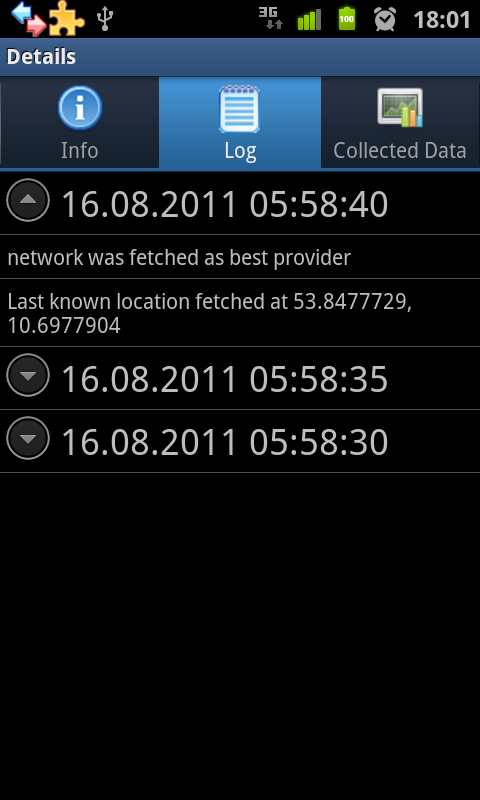
\includegraphics[width=5cm]{grafiken/log.png}
	\caption{Zugriffsprotokoll auf den LocationManager}
	\label{log_locationtracker}
\end{figure}

\begin{figure}[h!] 
	\centering
	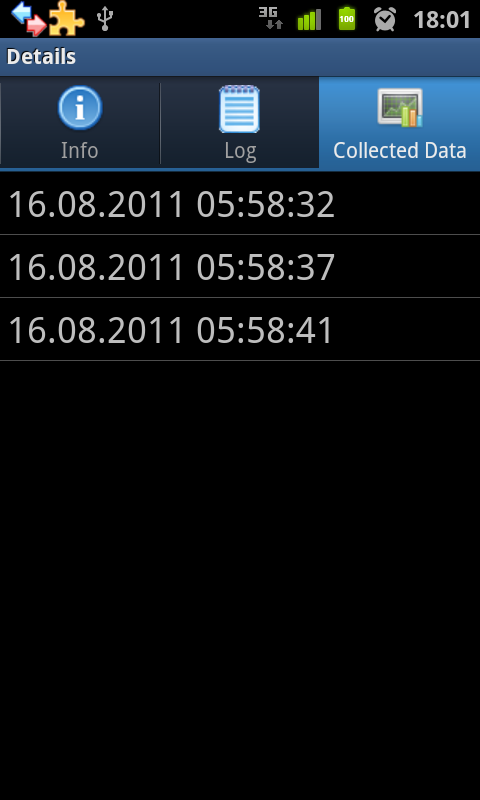
\includegraphics[width=5cm]{grafiken/collected_data_overview.png}
	\caption{�berblick �ber alle gesammelten Positionen}
	\label{collected_data_overview_locationtracker}
\end{figure}

\begin{figure}[h!] 
	\centering
	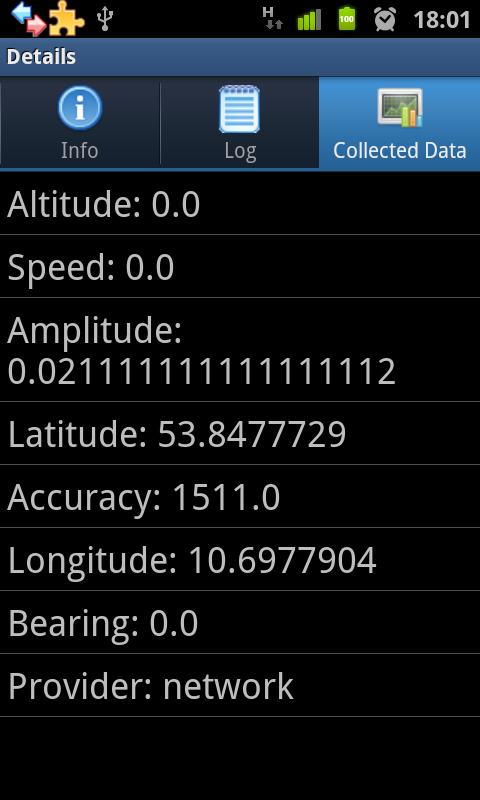
\includegraphics[width=5cm]{grafiken/collected_data_details.png}
	\caption{Detailierte Ansicht einer Position}
	\label{collected_data_details_locationtracker}
\end{figure}

Das Plug-In demonstriert somit, dass es mit dem {\em Mobile Data
Collection Framework} m�glich ist, Plug-Ins zu entwickeln, die
Positionsdaten sammeln k�nnen. Im n�chsten Abschnitt wird gezeigt, wie die
gesammelten Daten von einem Server empfangen, verarbeitet und visualisiert
werden k�nnen.

\subsection{Implementierung der Serverkomponente}
Bei der Implementierung der Serverkomponente wird als Ausgangspunkt die ``Hallo
Welt''-Serverkomponente verwendet. Diese wurde um eine Persistierungsschicht
erweitert und erlaubt die Visualisierung der Daten mit Hilfe einer
Web-Anwendung. Die Serverkomponente befindet sich im {\em
mdcf-locationtracker-remote}-Verzeichnis, des {\em Mobile Data
Collector}-Projektes.

\subsubsection{Persistierung der Daten}
Wie in Kapitel \ref{cha:leitfaden} beschrieben, werden nach dem Empfang, die
Daten an einen {\em TransferRequestProcessor} �bergeben. In der Klasse kann
z.~B. die Persistierung der Daten stattfinden. Bevor die Daten gespeichert
werden, sollte aber eine �berf�hrung des allgemeinen Datenformats des {\em Mobile Data Collection
Frameworks} in ein dom�nenspezifisches stattfinden. Eine �berf�hrung
des allgemeinen Datenformats in ein dom�nenspezifisches sowie die anschlie�ende
Speicherung, kann wie in Listing \ref{datenmapping} implementiert werden.

\begin{lstlisting}[label=datenmapping,
caption=TransferRequestProcessorImpl.java, language=java] 
package de.uniluebeck.itm.mdcf.remote.locationtracker.server;

import java.util.Iterator;
import java.util.List;

import com.google.common.base.Objects;
import com.google.inject.Inject;

import de.uniluebeck.itm.mdcf.remote.TransferRequestProcessor;
import de.uniluebeck.itm.mdcf.remote.locationtracker.server.domain.Location;
import de.uniluebeck.itm.mdcf.remote.locationtracker.server.domain.Participant;
import de.uniluebeck.itm.mdcf.remote.model.Node;
import de.uniluebeck.itm.mdcf.remote.model.TransferRequest;

public class TransferRequestProcessorImpl implements TransferRequestProcessor {
	
	private final ParticipantRepository repository;
	
	@Inject
	public TransferRequestProcessorImpl(
			ParticipantRepository repository) {
		this.repository = repository;
	}
	
	public void process(TransferRequest request) {
		String id = request.getId();
		Participant participant = Objects.firstNonNull(
			repository.findById(id), new Participant(id));
		
		Node workspace = request.getWorkspace();
		Iterator<Node> nodes = workspace.getNodes();
		List<Location> locations = participant.getLocations();
		while (nodes.hasNext()) {
			Node node = nodes.next();
			Location location = new Location();
			location.setTimestamp(node.getTimestamp());
			location.setLatitude(node.getProperty("Latitude")
				.getValue().getDouble());
			location.setLongitude(node.getProperty("Longitude")
				.getValue().getDouble());
			location.setAltitude(node.getProperty("Altitude")
				.getValue().getDouble());
			location.setBearing((float) node.getProperty("Bearing")
				.getValue().getDouble());
			location.setAccuracy((float) node.getProperty("Accuracy")
				.getValue().getDouble());
			location.setSpeed((float) node.getProperty("Speed")
				.getValue().getDouble());
			location.setProvider(node.getProperty("Provider")
				.getValue().getString());
			locations.add(location);
		}
		repository.persist(participant);
	}
}
\end{lstlisting}

In diesem Listing wird gezeigt, wie der empfangene {\em TransferRequest} auf
ein {\em Participant}-Objekt �bertragen werden kann. Ein {\em Participant}
stellt einen Benutzer des {\em Mobile Data Collector} dar. Die
Identifikation findet anhand der eindeutigen Benutzerkennung statt, welche �ber
die {\em getId}-Methode abgefragt werden kann. Sollte der {\em Participant}
bereits existierten, werden die gesammelten Daten, an den bereits existierenden
Benutzer ran gehangen, sonst wird ein neuer {\em Participant} erstellt. Das {\em
PersistentRepository} stellt die Datenbankabstraktionsschicht dar. In den darauf
folgenden Schritten werden die Daten aus dem {\em TransferRequest} an ein
entsprechendes {\em Location}-Objekt �bergeben und der {\em Participant} wird
gespeichert. Die Daten sind nun in einer Datenbank persistiert und stehen somit
anderen Anwendungen zur Verf�gung. In diesem Beispiel wurde zur Persistierung
der \acf{orm} {\em Hibernate} verwendet. Die Persistierungsmethode wird vom {\em
ParticipantRepsitory} abstrahiert. Durch die Abstraktion steht es dem Entwickler frei ein
beliebiges anderes Persistierungsframework zu verwenden.

\subsubsection{Visualisierung der Daten}
Als letzter Teil der Evaluation sollen die gespeicherten Daten visualisiert
werden. Da es sich um Positionsdaten handelt, bietet es sich an, die
Positionen eines Benutzers auf einer Karte zu visualisieren. Dadurch ist es
sehr einfach m�glich, die Daten zu evaluieren.

F�r die technische Realisierung bietet es sich an, auf bereits bestehende
Infrastruktur und Programmiersprachen zur�ckzugreifen. Da bisher nur die
Programmiersprache Java verwendet wurde und bereits ein Java Servlet-Container
zum Empfang der Daten vorhanden ist, eignet sich ein javabasiertes
Web-Framework am besten. In diesem Fall fiel die Wahl auf
das \acf{gwt}\cite{gwt}. Bei \acs{gwt} handelt es sich um einen
Java-zu-JavaScript-Compiler, der die Implementierung von Web-Anwendung in Java
erlaubt. Die clientseitige Ausf�hrung der Web-Anwendung findet nach der
Kompilierung nur noch in JavaScript statt. Zur Einbindung von Karten wurde die
Google Maps \acs{api} f�r \acs{gwt} verwendet\cite{gwtmaps}.

In Abbildung \ref{locationtrackermap} ist die Web-Anwendung dargestellt. Im
oberen Bereich befinden sich alle Bedienelemente. �ber die erste List-Box lassen
sich unterschiedliche Benutzer anhand ihrer eindeutigen Benutzerkennung
ausw�hlen. �ber die zweite List-Box lassen sich zu jedem Benutzer die
aufgenommenen Positionen ausw�hlen. Die daneben befindlichen Bedienelemente
dienen zur Navigation durch die Daten sowie einer Funktion zum automatischen
Durchlaufen der Positionen. Man kann dadurch die Bewegung eines Benutzers besser
verfolgen. Zu jeder Position werden au�erdem alle gesammelten Informationen
angezeigt. Der gr�ne Kreis gibt an, wie genau die Messung
war. In diesem Fall wurde die Messung auf 57 Meter genau durchgef�hrt, welches
sich in dem Radius des Kreises widerspiegelt.

\begin{figure}[h!] 
	\centering
	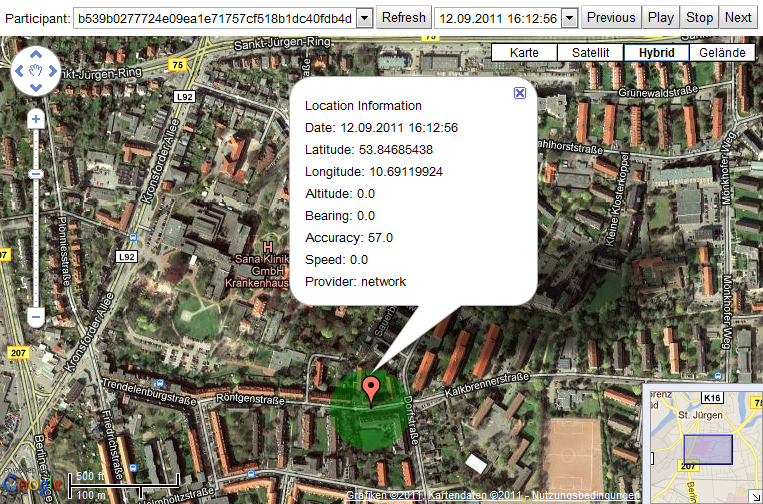
\includegraphics[width=13cm]{grafiken/locationtracker-remote_map.png}
	\caption{Location-Tracker-Datenvisualisierung}
	\label{locationtrackermap}
\end{figure}

Um die Web-Anwendung auf dem eigenen Computer zu starten, muss die {\em
persistence.xml} an die eigene Datenbank angepasst werden. Dann kann
Folgendes auf der Kommandozeile im {\em mdcf-locationtracker-remote}-Verzeichnis
ausgef�hrt werden.

\begin{lstlisting}[language=bash]
mvn gwt:run
\end{lstlisting}

Daraufhin startet der \acs{gwt} eigene Webserver sowie das
Servlet zum Empfang der Daten. Gibt man die entsprechende lokale IP-Adresse innerhalb der
Plug-In Konfiguration an, so kann der Webserver die Daten vom {\em Mobile Data
Collector} empfangen und �ber die Web-Anwendung darstellen.

\section{Plug-In zum Sammeln der Lautst�rke an der aktuellen Position}
Aufbauend auf dem in Abschnitt \ref{locationtracker} beschriebenen {\em
Location Tracker}, wird im Folgenden ein Plug-In entwickelt, das neben der
aktuellen Position auch die Lautst�rke speichert. Das Plug-In tr�gt den
Arbeitstitel {\em Noise Tracker}.

\subsection{Plug-In Anpassungen}
Das Plug-In befindet sich im {\em NoiseTrackerPlugin}-Verzeichnis. Es wird sich
im Folgenden auf dem im Verzeichnis befindlichen Quellcode bezogen.

Da der {\em Location Tracker} bereits die aktuelle Position bestimmt, muss noch
die aktuelle Lautst�rke ermittelt werden. Das ist in Listing \ref{messurenoise}
dargestellt.

\begin{lstlisting}[label=messurenoise,
caption=Lautst�rkenmessung, language=java] 
recorder = new MediaRecorder();
recorder.setAudioSource(MediaRecorder.AudioSource.MIC);
recorder.setOutputFormat(MediaRecorder.OutputFormat.THREE_GPP);
recorder.setAudioEncoder(MediaRecorder.AudioEncoder.AMR_NB);
recorder.setOutputFile("/dev/null");
recorder.prepare();
recorder.start();

double amplitude = 0.0;
for (int i = 0; i < 10; i++) {
	amplitude = getAmplitude();
	Thread.sleep(100);
}

recorder.stop();
recorder.release();
\end{lstlisting}

In dem Listing wird zuerst ein {\em MediaRecorder} erstellt. Der kann dazu
verwendet werden, um Audio- und Videoaufnahmen durchzuf�hren. In den darauf folgenden
Zeilen wird als Audioquelle das Mikrofon verwendet. Die Einstellungen zum
Ausgabeformat und Audio-Encoder sind zwar notwendig, aber
irrelevant, da wie in Zeile 5 angegeben alle Daten im {\em null-Device} gespeichert werden.
Durch die {\em prepare}- und {\em start}-Methode wird das Mikrofon reserviert
und die Aufnahme gestartet. Die Lautst�rke wird nun anhand der maximalen Amplitude
bestimmt, welchen �ber die {\em getAmplitude}-Methode abgefragt werden kann.
Damit die Methode einen brauchbaren Wert zur�ckliefert, muss f�r eine bestimmte
Zeitspanne eine Tonaufnahme erfolgen. In diesem Fall werden f�r eine Sekunde
lang, alle Umgebungsger�usche aufgenommen und die maximale Amplitude bestimmt.
Durch die {\em stop}- und {\em release}-Methode wird die Aufnahme angehalten und das
Mikrofon wieder freigegeben. Diese Art zur Lautst�rkenbestimmung wurde dem
Beispielprogramm {\em NoiseAlert} entnommen~\cite{noisealert}. Dabei ist zu
erw�hnen, dass die maximale Amplitude zwischen verschiedenen Ger�ten
variieren kann. Bei einer Auswertung ist deswegen eine Normalisierung
der Daten erforderlich.

Um die Amplitude zum bisherigen Datenmodell hinzuzuf�gen, ist die Zeile
aus Listing \ref{storeamplitude} hinzuzuf�gen.

\begin{lstlisting}[label=storeamplitude,
caption=Speichern der Ampltiude, language=java] 
node.setProperty("Amplitude", amplitude);
\end{lstlisting}

Als letzte Anpassung muss dem Plug-In noch die {\em Permission} zur Aufnahme von
Tonaufnahmen erhalten. Dazu muss die {\em AndroidManifest.xml} um die Zeile aus 
Listing \ref{recordaudio} erg�nzt werden.

\begin{lstlisting}[label=recordaudio,
caption=Permission f�r Tonaufnahmen, language=xml] 
<uses-permission
	android:name="android.permission.RECORD_AUDIO" />
\end{lstlisting}

Bei der Verwendung der {\em Permission} sei darauf hingewiesen, dass der
Benutzer wie in Abbildung \ref{activation_recordaudio_warning} eine Warnung bei der
Aktivierung erh�lt, da durch die Aufnahme von Ton personenbezogene Daten erhoben
werden k�nnen. Der {\em Mobile Data Collector} ist nicht in der Lage zu
protokollieren, was wann aufgenommen wurde, sondern kann nur das Resultat
speichern. Siehe hierzu auch Abschnitt \ref{problemsofimplementation}.

\begin{figure}[h!] 
	\centering
	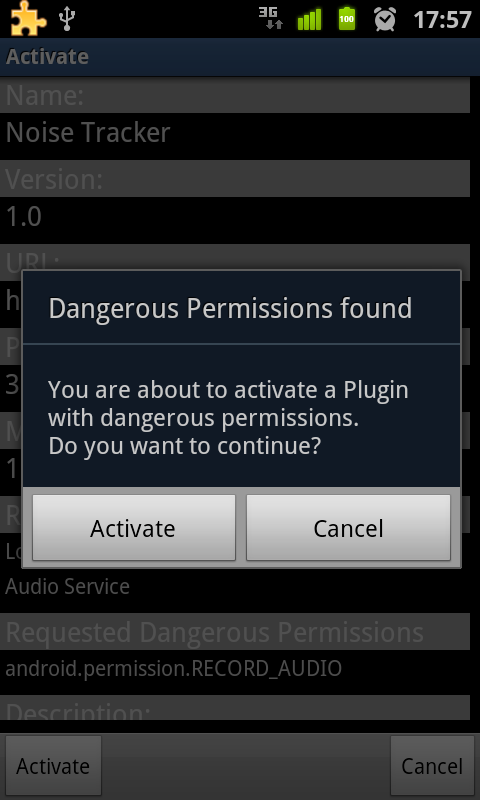
\includegraphics[width=5cm]{grafiken/activation_warning.png}
	\caption{Warnung bei der Aktivierung}
	\label{activation_recordaudio_warning}
\end{figure}

Das Plug-In ist jetzt vollst�ndig implementiert und kann zur Ermittlung der
Lautst�rke verwendet werden.

\subsection{Anpassungen der Serverkomponente}
Die Anpassungen an der Serverkomponente halten sich ebenfalls in Grenzen. Bei
der �bertragung des allgemeinen Datenmodells auf das dom�nenspezifische muss
entsprechend ein Attribut f�r die Amplitude vorgesehen werden.

Bei der Visualisierung wurde in diesem Fall nur ein weiteres Attribut bei der
Ausgabe aller Positionsdaten hinzugef�gt. Siehe hierzu Abbildung
\ref{noisetrackermap}.

\begin{figure}[h!] 
	\centering
	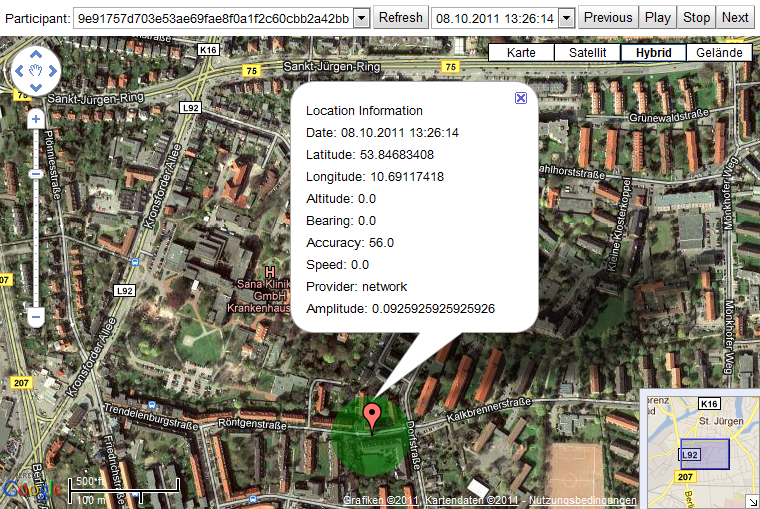
\includegraphics[width=13cm]{grafiken/noisetracker-remote_map.png}
	\caption{Noise-Tracker-Datenvisualisierung}
	\label{noisetrackermap}
\end{figure}

\section{Evaluationsergebnisse}
Als Ergebnis der Evaluation l�sst sich folgendes Festhalten:

\begin{itemize}
  \item Die Erstellung von Plug-Ins f�r reale Anwendungsszenarien, z.~B. die
  Erfassung der aktuellen Positionen und Lautst�rke, ist
  mit dem {\em Mobile Data Collection Framework} m�glich.
  \item Das allgemeine Datenformat erlaubt das Speichern von beliebigen
  Informationen und schr�nkt einen Plug-In Entwickler nur bedingt ein.
  \item Bestehende Plug-Ins lassen sich leicht an neuen Anforderungen anpassen
  bzw. erweitern.
  \item Bei der Verwendung von Android-{\em Permissions} die den Zugriff auf
  personenbezogene Daten erm�glichen, wird der Benutzer vor der Aktivierung
  gewarnt.
  \item Die Zugriffe auf die sicheren Android System Services werden
  protokolliert und sind, wie die vom Plug-In gesammelten Daten, zu jedem
  Zeitpunkt einsehbar.
  \item Die gesammelten Daten lassen sich anonym an externe Server �bertragen
  und persistieren. Die serverseitige Persistenzart ist frei w�hlbar.
  \item Die Visualisierung hat gezeigt, dass die Daten auch verwertbar sind. Der
  Visualisierung sind hierbei keine Grenzen gesetzt.
  \item Es ist zurzeit nicht m�glich, die Aufnahme von Ton und Video �ber den
  {\em Mobile Data Collector} zu protokollieren. Der Benutzer wird aber gewarnt
  sollte ein Plug-In dieses versuchen.
\end{itemize}

Abschlie�end l�sst sich festhalten, dass die in der Anforderungsanalyse und dem
Konzept definierten Anforderungen fast vollst�ndig realisiert wurden, mit
Ausnahme der Protokollierung beim Zugriff auf Ton- und Videodaten.
	\chapterfin
	\chapter{Zusammenfassung und Ausblick}
\label{cha:zusammenfassung}
Im Rahmen dieser Masterarbeit wurde ein dreiteiliges Software-System
entwickelt, dass das transparente und anonyme Sammeln von Sensordaten auf
Android-Smartphones erm�glicht. Diese drei Teile sind der {\em Mobile Data
Collector}, das {\em Mobile Data Collection Framework} sowie ein
serverseitiges Framework zum Empfang der gesammelten Sensordaten.

Kern der Arbeit war es eine vertrauensw�rdige Plattform zu schaffen, f�r die
Entwicklung von Plug-Ins zum Sammeln von Sensordaten (potenziell
personenbezogenen), die es aber dem Benutzer erlaubt, alle Aktivit�ten und
gesammelten Daten des Plug-Ins einzusehen. Durch diese Transparenz sollen
Smartphone-Besitzer, Vertrauen in den {\em Mobile Data Collector} erlangen und
einen Teil ihrer pers�nlichen Daten an Plug-Ins preisgeben, ohne einen direkten
Mehrwert von den Plug-Ins zu erhalten.

Die Realisierung der erarbeiteten Anforderungen und Konzepte hat eine
erweiterbare Android-Anwendung hervorgebracht, die das bereits existierende
Security-System von Android durch Monitoring-Mechanismen erweitert. Der {\em
Mobile Data Collector} l�sst sich durch Sensordaten sammelnde Plug-Ins
erweitern, die mit dem {\em Mobile Data Collection Framework} entwickelt werden.
Vor der ersten Ausf�hrung eines Plug-In werden diese analysiert und der Benutzer
wird �ber Gefahren, die vom Plug-In ausgehen k�nnen informiert. Der Benutzer
beh�lt hierbei, wie im Konzept beschrieben, immer die Kontrolle �ber seine
Daten. Er kann die Ausf�hrungszeit eines Plug-In bestimmen und wird �ber die
Ausf�hrung informiert, kann einsehen, auf welche personenbezogenen Daten
zugegriffen wurden sowie welche Daten an den Plug-In spezifischen Server
�bertragen werden sollen. Die Anonymit�t des Benutzers wird dadurch
sichergestellt, dass das Framework den Zugriff auf eindeutige Benutzerdaten gar
nicht erst zur Verf�gung stellt. Die bei der �bertragung verwendete eindeutige
Benutzerkennung erlaubt zwar die Zuordnung von Daten zu bereits empfangen
Daten, erlaubt aber nicht die Zuordnung zu realen Personen.

Die Evaluation hat gezeigt, dass sich mit dem {\em Mobile Data Collection
Framework} Plug-Ins f�r reale Anwendungsszenarien entwickeln lassen. So ist die
Aufnahme von Positionsdaten, die wohl wichtigste Art von Daten im Bereich der
mobilen Datenerfassung, relativ einfach m�glich. Auch lassen sich diese Daten
einfach um zus�tzliche Daten erweitern. Hierbei wurde bewusst darauf geachtet,
dem Entwickler m�glichst nicht bei der Entwicklung von Plug-Ins einzuschr�nken.

Die Evaluation zeigt aber auch die zurzeit bestehenden Monitoring-Grenzen des
{\em Mobile Data Collector}. So ist ein Monitoring der Kamera und des Mikrofons
nicht bzw. nur mit relativ gro�em Aufwand m�glich. Dieses Problem l�sst sich am
besten durch die Einf�hrung von OSGi l�sen. Hierbei bleibt aber abzuwarten bis
Frameworks wie Dynamix den n�tigen Reifegrad erreicht haben, um diese im
produktiven Einsatz zu verwenden.

Das zuk�nftige Anwendungsgebiet des {\em Mobile Data Collector} liegen in
erster Linie im Bereich der Forschung. Hier existiert eine Vielzahl von
Projekten, die auf die Erhebung von personenbezogenen Daten angewiesen sind.
Aber auch in der Industrie ergeben sich viele Anwendungsfelder. Vor
allen Dingen kann der {\em Mobile Data Collector} eine M�glichkeit schaffen, an
Daten zu gelangen, die normalerweise nur Mobilfunkunternehmen oder
Smartphone-Betriebssystemhersteller wie Google oder Apple vorbehalten sind.

	\chapterfin

%---------------------------------------------------------------------------
% Anhang
%---------------------------------------------------------------------------
	\appendix
		
		%---------------------------------------------------------------------------

	\addcontentsline{toc}{chapter}{Verzeichnisse}

		%---------------------------------------------------------------------------
		\addcontentsline{toc}{section}{Abbildungsverzeichnis}
		\listoffigures
		\sectionfin		
		%---------------------------------------------------------------------------
	
		%---------------------------------------------------------------------------
		%\addcontentsline{toc}{section}{Abk�rzungsverzeichnis}
		%If you are using e. g. the documentclass book with page style headings you
		%should also take care of correct headings:	
		%\markboth{Abk�rzungsverzechnis}{Abk�rzungsverzechnis}
		%\printnomenclature
		%\sectionfin
		%Abk�rzungsverzeichnis
		\phantomsection
		\addcontentsline{toc}{section}{Abk�rzungsverzeichnis}
		\markboth{Abk�rzungsverzechnis}{Abk�rzungsverzechnis}
		\section*{Abk�rzungsverzeichnis}
		\begin{acronym}[MMORPG]
		\setlength{\itemsep}{-\parsep}
		\renewcommand{\bflabel}[1]{\normalfont{\normalsize{\textbf{#1}}}\hfill}
		\acro{aidl}[AIDL]{Android Interface Definition Language}
\acro{api}[API]{Application Programming Interface}
\acro{db4o}[db4o]{database for objects}
\acro{gps}[GPS]{Global Positioning System}
\acro{gsm}[GSM]{Global System for Mobile Communications}
\acro{gwt}[GWT]{Google Web Toolkit}
\acro{http}[HTTP]{Hypertext Transfer Protocol}
\acro{ide}[IDE]{Integrated Development Environment}
\acro{idl}[IDL]{Interface Definition Language}
\acro{imsi}[IMSI]{International Mobile Subscriber Identity}
\acro{ipc}[IPC]{Inter Process Communication}
\acro{itm}[ITM]{Institut f�r Telematik}
\acro{lan}[LAN]{Local Area Network}
\acro{jar}[JAR]{Java Archive}
\acro{jcr}[JCR]{Java Content Repository}
\acro{json}[JSON]{Java Script Object Notation}
\acro{jsr}[JSR]{Java Specification Request}
\acro{orm}[ORM]{Objekt Relationale Mapper}
\acro{osgi}[OSGi]{Open Services Gateway initiative}
\acro{rest}[REST]{Representational State Transfer}
\acro{sql}[SQL]{Structured Query Language}
\acro{qbe}[QBE]{Query By Example}
\acro{pojo}[POJO]{Plain Old Java Object}
\acro{sdk}[SDK]{Software Development Kit}
\acro{sha}[SHA]{Secure Hash Algorithm}
\acro{umts}[UMTS]{Universal Mobile Telecommunications System}
\acro{vm}[VM]{Virtual Machine}
\acro{xml}[XML]{Extensible Markup Language}
		\end{acronym}
		\sectionfin
		%---------------------------------------------------------------------------
	
		%---------------------------------------------------------------------------
		%---------------------------------------------------------------------------
		\renewcommand\bibname{Bibliographie}
		\addcontentsline{toc}{section}{Bibliographie}
		\bibliographystyle{acm}
		\bibliography{quellen/master}

		\chapterfin

\end{document}
